\documentclass[twoside]{book}

% Packages required by doxygen
\usepackage{fixltx2e}
\usepackage{calc}
\usepackage{doxygen}
\usepackage[export]{adjustbox} % also loads graphicx
\usepackage{graphicx}
\usepackage[utf8]{inputenc}
\usepackage{makeidx}
\usepackage{multicol}
\usepackage{multirow}
\PassOptionsToPackage{warn}{textcomp}
\usepackage{textcomp}
\usepackage[nointegrals]{wasysym}
\usepackage[table]{xcolor}

% Font selection
\usepackage[T1]{fontenc}
\usepackage[scaled=.90]{helvet}
\usepackage{courier}
\usepackage{amssymb}
\usepackage{sectsty}
\renewcommand{\familydefault}{\sfdefault}
\allsectionsfont{%
  \fontseries{bc}\selectfont%
  \color{darkgray}%
}
\renewcommand{\DoxyLabelFont}{%
  \fontseries{bc}\selectfont%
  \color{darkgray}%
}
\newcommand{\+}{\discretionary{\mbox{\scriptsize$\hookleftarrow$}}{}{}}

% Page & text layout
\usepackage{geometry}
\geometry{%
  a4paper,%
  top=2.5cm,%
  bottom=2.5cm,%
  left=2.5cm,%
  right=2.5cm%
}
\tolerance=750
\hfuzz=15pt
\hbadness=750
\setlength{\emergencystretch}{15pt}
\setlength{\parindent}{0cm}
\setlength{\parskip}{0.2cm}
\makeatletter
\renewcommand{\paragraph}{%
  \@startsection{paragraph}{4}{0ex}{-1.0ex}{1.0ex}{%
    \normalfont\normalsize\bfseries\SS@parafont%
  }%
}
\renewcommand{\subparagraph}{%
  \@startsection{subparagraph}{5}{0ex}{-1.0ex}{1.0ex}{%
    \normalfont\normalsize\bfseries\SS@subparafont%
  }%
}
\makeatother

% Headers & footers
\usepackage{fancyhdr}
\pagestyle{fancyplain}
\fancyhead[LE]{\fancyplain{}{\bfseries\thepage}}
\fancyhead[CE]{\fancyplain{}{}}
\fancyhead[RE]{\fancyplain{}{\bfseries\leftmark}}
\fancyhead[LO]{\fancyplain{}{\bfseries\rightmark}}
\fancyhead[CO]{\fancyplain{}{}}
\fancyhead[RO]{\fancyplain{}{\bfseries\thepage}}
\fancyfoot[LE]{\fancyplain{}{}}
\fancyfoot[CE]{\fancyplain{}{}}
\fancyfoot[RE]{\fancyplain{}{\bfseries\scriptsize Generated on Sat Jun 20 2015 18\+:44\+:10 for Summarizer by Doxygen }}
\fancyfoot[LO]{\fancyplain{}{\bfseries\scriptsize Generated on Sat Jun 20 2015 18\+:44\+:10 for Summarizer by Doxygen }}
\fancyfoot[CO]{\fancyplain{}{}}
\fancyfoot[RO]{\fancyplain{}{}}
\renewcommand{\footrulewidth}{0.4pt}
\renewcommand{\chaptermark}[1]{%
  \markboth{#1}{}%
}
\renewcommand{\sectionmark}[1]{%
  \markright{\thesection\ #1}%
}

% Indices & bibliography
\usepackage{natbib}
\usepackage[titles]{tocloft}
\setcounter{tocdepth}{3}
\setcounter{secnumdepth}{5}
\makeindex

% Hyperlinks (required, but should be loaded last)
\usepackage{ifpdf}
\ifpdf
  \usepackage[pdftex,pagebackref=true]{hyperref}
\else
  \usepackage[ps2pdf,pagebackref=true]{hyperref}
\fi
\hypersetup{%
  colorlinks=true,%
  linkcolor=blue,%
  citecolor=blue,%
  unicode%
}

% Custom commands
\newcommand{\clearemptydoublepage}{%
  \newpage{\pagestyle{empty}\cleardoublepage}%
}


%===== C O N T E N T S =====

\begin{document}

% Titlepage & ToC
\hypersetup{pageanchor=false,
             bookmarks=true,
             bookmarksnumbered=true,
             pdfencoding=unicode
            }
\pagenumbering{roman}
\begin{titlepage}
\vspace*{7cm}
\begin{center}%
{\Large Summarizer }\\
\vspace*{1cm}
{\large Generated by Doxygen 1.8.9.1}\\
\vspace*{0.5cm}
{\small Sat Jun 20 2015 18:44:10}\\
\end{center}
\end{titlepage}
\clearemptydoublepage
\tableofcontents
\clearemptydoublepage
\pagenumbering{arabic}
\hypersetup{pageanchor=true}

%--- Begin generated contents ---
\chapter{Hierarchical Index}
\section{Class Hierarchy}
This inheritance list is sorted roughly, but not completely, alphabetically\+:\begin{DoxyCompactList}
\item \contentsline{section}{config}{\pageref{classconfig}}{}
\item \contentsline{section}{Lexical\+Chain}{\pageref{classLexicalChain}}{}
\item \contentsline{section}{related\+\_\+words}{\pageref{structrelated__words}}{}
\item \contentsline{section}{Relation}{\pageref{classRelation}}{}
\begin{DoxyCompactList}
\item \contentsline{section}{Hypernymy}{\pageref{classHypernymy}}{}
\item \contentsline{section}{Same\+Coref\+Group}{\pageref{classSameCorefGroup}}{}
\item \contentsline{section}{Same\+Word}{\pageref{classSameWord}}{}
\end{DoxyCompactList}
\item \contentsline{section}{Summarizer}{\pageref{classSummarizer}}{}
\item \contentsline{section}{word\+\_\+pos}{\pageref{structword__pos}}{}
\end{DoxyCompactList}

\chapter{Class Index}
\section{Class List}
Here are the classes, structs, unions and interfaces with brief descriptions\+:\begin{DoxyCompactList}
\item\contentsline{section}{\hyperlink{classconfig}{config} \\*Class config implements a set of specific options for the N\+L\+P analyzer, providing a C++ wrapper to libcfg+ library }{\pageref{classconfig}}{}
\item\contentsline{section}{\hyperlink{classHypernymy}{Hypernymy} \\*Class \hyperlink{classHypernymy}{Hypernymy} represents the hypernymy relation\+: two words are related if one is an hypernymy of the other and the hypernymy depth is smaller or equal than a given maximum }{\pageref{classHypernymy}}{}
\item\contentsline{section}{\hyperlink{classLexicalChain}{Lexical\+Chain} \\*Class \hyperlink{classLexicalChain}{Lexical\+Chain} represents a lexical chain and computes words and stores (or not) them into the structures }{\pageref{classLexicalChain}}{}
\item\contentsline{section}{\hyperlink{structrelated__words}{related\+\_\+words} \\*Struct that represents a relationship between two words }{\pageref{structrelated__words}}{}
\item\contentsline{section}{\hyperlink{classRelation}{Relation} \\*Class \hyperlink{classRelation}{Relation} is a non-\/instantiable class which defines many virtual methods to check if a word is compatible with the \hyperlink{classRelation}{Relation} or if a word can be stored in the structures of a lexical chain }{\pageref{classRelation}}{}
\item\contentsline{section}{\hyperlink{classSameCorefGroup}{Same\+Coref\+Group} \\*Class \hyperlink{classSameCorefGroup}{Same\+Coref\+Group} represents the same coreference group relation\+: two words are related if they are in the same coreference group }{\pageref{classSameCorefGroup}}{}
\item\contentsline{section}{\hyperlink{classSameWord}{Same\+Word} \\*Class \hyperlink{classSameWord}{Same\+Word} represents the same word relation\+: two words are related if they are the same word }{\pageref{classSameWord}}{}
\item\contentsline{section}{\hyperlink{classSummarizer}{Summarizer} \\*\hyperlink{classSummarizer}{Summarizer} class summarizes a document using the lexical chains method }{\pageref{classSummarizer}}{}
\item\contentsline{section}{\hyperlink{structword__pos}{word\+\_\+pos} \\*Struct that allow us to compare words easily }{\pageref{structword__pos}}{}
\end{DoxyCompactList}

\chapter{File Index}
\section{File List}
Here is a list of all files with brief descriptions\+:\begin{DoxyCompactList}
\item\contentsline{section}{\hyperlink{config_8h}{config.\+h} }{\pageref{config_8h}}{}
\item\contentsline{section}{\hyperlink{LexicalChain_8cc}{Lexical\+Chain.\+cc} }{\pageref{LexicalChain_8cc}}{}
\item\contentsline{section}{\hyperlink{LexicalChain_8h}{Lexical\+Chain.\+h} }{\pageref{LexicalChain_8h}}{}
\item\contentsline{section}{\hyperlink{Relation_8cc}{Relation.\+cc} }{\pageref{Relation_8cc}}{}
\item\contentsline{section}{\hyperlink{Relation_8h}{Relation.\+h} }{\pageref{Relation_8h}}{}
\item\contentsline{section}{\hyperlink{Summarizer_8cc}{Summarizer.\+cc} }{\pageref{Summarizer_8cc}}{}
\item\contentsline{section}{\hyperlink{Summarizer_8h}{Summarizer.\+h} }{\pageref{Summarizer_8h}}{}
\item\contentsline{section}{\hyperlink{summarizer__main_8cc}{summarizer\+\_\+main.\+cc} }{\pageref{summarizer__main_8cc}}{}
\end{DoxyCompactList}

\chapter{Class Documentation}
\hypertarget{classconfig}{}\section{config Class Reference}
\label{classconfig}\index{config@{config}}


Class config implements a set of specific options for the N\+L\+P analyzer, providing a C++ wrapper to libcfg+ library.  




{\ttfamily \#include $<$config.\+h$>$}



Collaboration diagram for config\+:\nopagebreak
\begin{figure}[H]
\begin{center}
\leavevmode
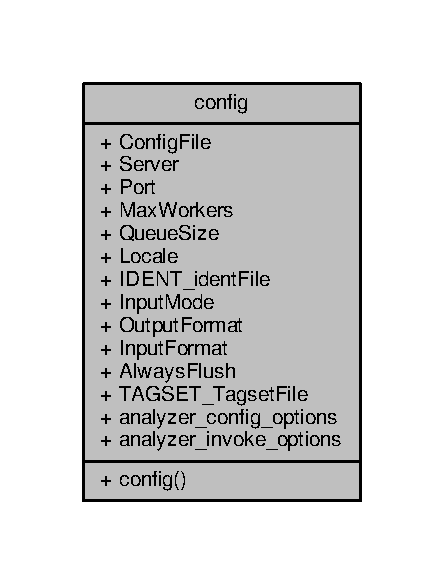
\includegraphics[width=213pt]{classconfig__coll__graph}
\end{center}
\end{figure}
\subsection*{Public Member Functions}
\begin{DoxyCompactItemize}
\item 
\hyperlink{classconfig_afe4a0fda7bf097bd04d713c06797e1f1}{config} (int ac, char $\ast$$\ast$av)
\begin{DoxyCompactList}\small\item\em constructor \end{DoxyCompactList}\end{DoxyCompactItemize}
\subsection*{Public Attributes}
\begin{DoxyCompactItemize}
\item 
std\+::string \hyperlink{classconfig_a24ba112bf45f600af2f79352b1c26646}{Config\+File}
\item 
bool \hyperlink{classconfig_a8868de72bdafb627b21b7f20e16ebf9e}{Server}
\begin{DoxyCompactList}\small\item\em Server mode on/off. \end{DoxyCompactList}\item 
int \hyperlink{classconfig_a05e9c81408b74459038340658bcd3a20}{Port}
\begin{DoxyCompactList}\small\item\em port number for server mode \end{DoxyCompactList}\item 
int \hyperlink{classconfig_a8771443c351f1d07be7eccc02beb8fff}{Max\+Workers}
\begin{DoxyCompactList}\small\item\em Maximum number of workers to fork (i.\+e. number of simultaneously atended clients) \end{DoxyCompactList}\item 
int \hyperlink{classconfig_ab690d59ef9d289198d2676ddc6bd5772}{Queue\+Size}
\begin{DoxyCompactList}\small\item\em Size of socket queue (number of clients waiting to be atended without being rejected) \end{DoxyCompactList}\item 
std\+::wstring \hyperlink{classconfig_a850a92a12eacd1bfee3f917792463b3f}{Locale}
\begin{DoxyCompactList}\small\item\em Locale of text to process. \end{DoxyCompactList}\item 
std\+::wstring \hyperlink{classconfig_a66b67d42d16146ebcc7f7bc355c5b60c}{I\+D\+E\+N\+T\+\_\+ident\+File}
\begin{DoxyCompactList}\small\item\em Configuration file for language identifier. \end{DoxyCompactList}\item 
\hyperlink{config_8h_ad5cac7b85d200232841f3f0a31bea5c1}{Input\+Modes} \hyperlink{classconfig_a081f4b86bc4315514b3693da987da11f}{Input\+Mode}
\begin{DoxyCompactList}\small\item\em Mode used to process input\+: D\+O\+C\+: load a document, then process it. \end{DoxyCompactList}\item 
\hyperlink{config_8h_a3f8677a5e7c7cdae9eae3f84e38bd5bd}{Output\+Formats} \hyperlink{classconfig_a79e21d6098e5fd1bfe615e2fef84a99f}{Output\+Format}
\begin{DoxyCompactList}\small\item\em Selected input and output format. \end{DoxyCompactList}\item 
\hyperlink{config_8h_aa29a34e3d6e44b1b5d909fb8cfcfdfb6}{Input\+Formats} \hyperlink{classconfig_ab66ebbcc7f73de39355cdf724cd644e6}{Input\+Format}
\item 
bool \hyperlink{classconfig_a604dde733e96d20cb065e2d39f8fe0e7}{Always\+Flush}
\begin{DoxyCompactList}\small\item\em whether splitter buffer must be flushed at each line \end{DoxyCompactList}\item 
std\+::wstring \hyperlink{classconfig_a6f42f7c1c60685d9b223fa9dc717a947}{T\+A\+G\+S\+E\+T\+\_\+\+Tagset\+File}
\begin{DoxyCompactList}\small\item\em Tagset to use for shortening tags in output. \end{DoxyCompactList}\item 
analyzer\+::config\+\_\+options \hyperlink{classconfig_a41502293ebef90c329451672bd879764}{analyzer\+\_\+config\+\_\+options}
\item 
analyzer\+::invoke\+\_\+options \hyperlink{classconfig_a0e4c6bbdd48bd59be36052970af2abff}{analyzer\+\_\+invoke\+\_\+options}
\end{DoxyCompactItemize}


\subsection{Detailed Description}
Class config implements a set of specific options for the N\+L\+P analyzer, providing a C++ wrapper to libcfg+ library. 

\subsection{Constructor \& Destructor Documentation}
\hypertarget{classconfig_afe4a0fda7bf097bd04d713c06797e1f1}{}\index{config@{config}!config@{config}}
\index{config@{config}!config@{config}}
\subsubsection[{config}]{\setlength{\rightskip}{0pt plus 5cm}config\+::config (
\begin{DoxyParamCaption}
\item[{int}]{ac, }
\item[{char $\ast$$\ast$}]{av}
\end{DoxyParamCaption}
)\hspace{0.3cm}{\ttfamily [inline]}}\label{classconfig_afe4a0fda7bf097bd04d713c06797e1f1}


constructor 



\subsection{Member Data Documentation}
\hypertarget{classconfig_a604dde733e96d20cb065e2d39f8fe0e7}{}\index{config@{config}!Always\+Flush@{Always\+Flush}}
\index{Always\+Flush@{Always\+Flush}!config@{config}}
\subsubsection[{Always\+Flush}]{\setlength{\rightskip}{0pt plus 5cm}bool config\+::\+Always\+Flush}\label{classconfig_a604dde733e96d20cb065e2d39f8fe0e7}


whether splitter buffer must be flushed at each line 

\hypertarget{classconfig_a41502293ebef90c329451672bd879764}{}\index{config@{config}!analyzer\+\_\+config\+\_\+options@{analyzer\+\_\+config\+\_\+options}}
\index{analyzer\+\_\+config\+\_\+options@{analyzer\+\_\+config\+\_\+options}!config@{config}}
\subsubsection[{analyzer\+\_\+config\+\_\+options}]{\setlength{\rightskip}{0pt plus 5cm}analyzer\+::config\+\_\+options config\+::analyzer\+\_\+config\+\_\+options}\label{classconfig_a41502293ebef90c329451672bd879764}
\hypertarget{classconfig_a0e4c6bbdd48bd59be36052970af2abff}{}\index{config@{config}!analyzer\+\_\+invoke\+\_\+options@{analyzer\+\_\+invoke\+\_\+options}}
\index{analyzer\+\_\+invoke\+\_\+options@{analyzer\+\_\+invoke\+\_\+options}!config@{config}}
\subsubsection[{analyzer\+\_\+invoke\+\_\+options}]{\setlength{\rightskip}{0pt plus 5cm}analyzer\+::invoke\+\_\+options config\+::analyzer\+\_\+invoke\+\_\+options}\label{classconfig_a0e4c6bbdd48bd59be36052970af2abff}
\hypertarget{classconfig_a24ba112bf45f600af2f79352b1c26646}{}\index{config@{config}!Config\+File@{Config\+File}}
\index{Config\+File@{Config\+File}!config@{config}}
\subsubsection[{Config\+File}]{\setlength{\rightskip}{0pt plus 5cm}std\+::string config\+::\+Config\+File}\label{classconfig_a24ba112bf45f600af2f79352b1c26646}
\hypertarget{classconfig_a66b67d42d16146ebcc7f7bc355c5b60c}{}\index{config@{config}!I\+D\+E\+N\+T\+\_\+ident\+File@{I\+D\+E\+N\+T\+\_\+ident\+File}}
\index{I\+D\+E\+N\+T\+\_\+ident\+File@{I\+D\+E\+N\+T\+\_\+ident\+File}!config@{config}}
\subsubsection[{I\+D\+E\+N\+T\+\_\+ident\+File}]{\setlength{\rightskip}{0pt plus 5cm}std\+::wstring config\+::\+I\+D\+E\+N\+T\+\_\+ident\+File}\label{classconfig_a66b67d42d16146ebcc7f7bc355c5b60c}


Configuration file for language identifier. 

\hypertarget{classconfig_ab66ebbcc7f73de39355cdf724cd644e6}{}\index{config@{config}!Input\+Format@{Input\+Format}}
\index{Input\+Format@{Input\+Format}!config@{config}}
\subsubsection[{Input\+Format}]{\setlength{\rightskip}{0pt plus 5cm}{\bf Input\+Formats} config\+::\+Input\+Format}\label{classconfig_ab66ebbcc7f73de39355cdf724cd644e6}
\hypertarget{classconfig_a081f4b86bc4315514b3693da987da11f}{}\index{config@{config}!Input\+Mode@{Input\+Mode}}
\index{Input\+Mode@{Input\+Mode}!config@{config}}
\subsubsection[{Input\+Mode}]{\setlength{\rightskip}{0pt plus 5cm}{\bf Input\+Modes} config\+::\+Input\+Mode}\label{classconfig_a081f4b86bc4315514b3693da987da11f}


Mode used to process input\+: D\+O\+C\+: load a document, then process it. 

C\+O\+R\+P\+U\+S\+: infinite sentence-\/by-\/sentnce processing \hypertarget{classconfig_a850a92a12eacd1bfee3f917792463b3f}{}\index{config@{config}!Locale@{Locale}}
\index{Locale@{Locale}!config@{config}}
\subsubsection[{Locale}]{\setlength{\rightskip}{0pt plus 5cm}std\+::wstring config\+::\+Locale}\label{classconfig_a850a92a12eacd1bfee3f917792463b3f}


Locale of text to process. 

\hypertarget{classconfig_a8771443c351f1d07be7eccc02beb8fff}{}\index{config@{config}!Max\+Workers@{Max\+Workers}}
\index{Max\+Workers@{Max\+Workers}!config@{config}}
\subsubsection[{Max\+Workers}]{\setlength{\rightskip}{0pt plus 5cm}int config\+::\+Max\+Workers}\label{classconfig_a8771443c351f1d07be7eccc02beb8fff}


Maximum number of workers to fork (i.\+e. number of simultaneously atended clients) 

\hypertarget{classconfig_a79e21d6098e5fd1bfe615e2fef84a99f}{}\index{config@{config}!Output\+Format@{Output\+Format}}
\index{Output\+Format@{Output\+Format}!config@{config}}
\subsubsection[{Output\+Format}]{\setlength{\rightskip}{0pt plus 5cm}{\bf Output\+Formats} config\+::\+Output\+Format}\label{classconfig_a79e21d6098e5fd1bfe615e2fef84a99f}


Selected input and output format. 

\hypertarget{classconfig_a05e9c81408b74459038340658bcd3a20}{}\index{config@{config}!Port@{Port}}
\index{Port@{Port}!config@{config}}
\subsubsection[{Port}]{\setlength{\rightskip}{0pt plus 5cm}int config\+::\+Port}\label{classconfig_a05e9c81408b74459038340658bcd3a20}


port number for server mode 

\hypertarget{classconfig_ab690d59ef9d289198d2676ddc6bd5772}{}\index{config@{config}!Queue\+Size@{Queue\+Size}}
\index{Queue\+Size@{Queue\+Size}!config@{config}}
\subsubsection[{Queue\+Size}]{\setlength{\rightskip}{0pt plus 5cm}int config\+::\+Queue\+Size}\label{classconfig_ab690d59ef9d289198d2676ddc6bd5772}


Size of socket queue (number of clients waiting to be atended without being rejected) 

\hypertarget{classconfig_a8868de72bdafb627b21b7f20e16ebf9e}{}\index{config@{config}!Server@{Server}}
\index{Server@{Server}!config@{config}}
\subsubsection[{Server}]{\setlength{\rightskip}{0pt plus 5cm}bool config\+::\+Server}\label{classconfig_a8868de72bdafb627b21b7f20e16ebf9e}


Server mode on/off. 

\hypertarget{classconfig_a6f42f7c1c60685d9b223fa9dc717a947}{}\index{config@{config}!T\+A\+G\+S\+E\+T\+\_\+\+Tagset\+File@{T\+A\+G\+S\+E\+T\+\_\+\+Tagset\+File}}
\index{T\+A\+G\+S\+E\+T\+\_\+\+Tagset\+File@{T\+A\+G\+S\+E\+T\+\_\+\+Tagset\+File}!config@{config}}
\subsubsection[{T\+A\+G\+S\+E\+T\+\_\+\+Tagset\+File}]{\setlength{\rightskip}{0pt plus 5cm}std\+::wstring config\+::\+T\+A\+G\+S\+E\+T\+\_\+\+Tagset\+File}\label{classconfig_a6f42f7c1c60685d9b223fa9dc717a947}


Tagset to use for shortening tags in output. 



The documentation for this class was generated from the following file\+:\begin{DoxyCompactItemize}
\item 
\hyperlink{config_8h}{config.\+h}\end{DoxyCompactItemize}

\hypertarget{classHypernymy}{}\section{Hypernymy Class Reference}
\label{classHypernymy}\index{Hypernymy@{Hypernymy}}


Class \hyperlink{classHypernymy}{Hypernymy} represents the hypernymy relation\+: two words are related if one is an hypernymy of the other and the hypernymy depth is smaller or equal than a given maximum.  




{\ttfamily \#include $<$Relation.\+h$>$}



Inheritance diagram for Hypernymy\+:\nopagebreak
\begin{figure}[H]
\begin{center}
\leavevmode
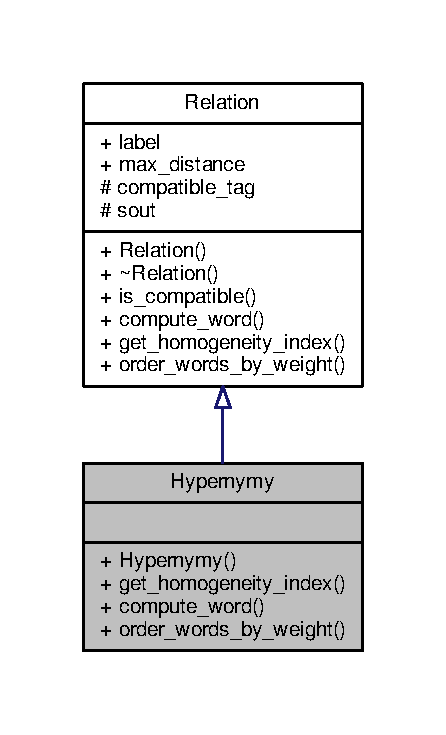
\includegraphics[width=214pt]{classHypernymy__inherit__graph}
\end{center}
\end{figure}


Collaboration diagram for Hypernymy\+:\nopagebreak
\begin{figure}[H]
\begin{center}
\leavevmode
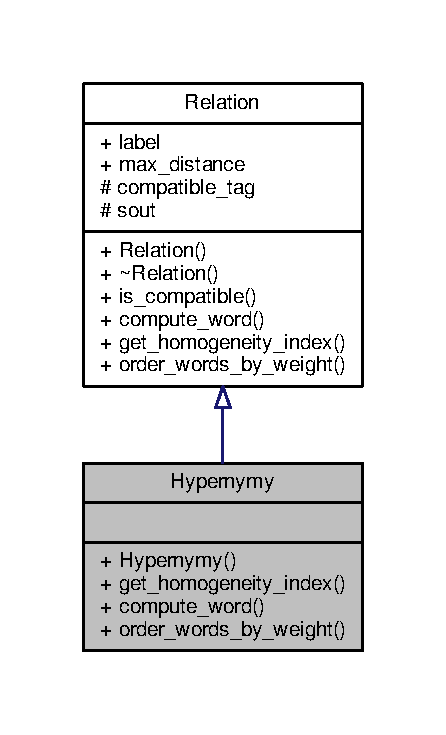
\includegraphics[width=214pt]{classHypernymy__coll__graph}
\end{center}
\end{figure}
\subsection*{Public Member Functions}
\begin{DoxyCompactItemize}
\item 
\hyperlink{classHypernymy_a763e43dbe511ef68413683bef8203937}{Hypernymy} (int k, double alpha, const std\+::wstring \&semfile, std\+::wostream \&\hyperlink{classRelation_a44deec0ee05d803ea23e14520fd57a75}{sout})
\begin{DoxyCompactList}\small\item\em Constructor. \end{DoxyCompactList}\item 
double \hyperlink{classHypernymy_a597074abd7795e114d13783677e55e20}{get\+\_\+homogeneity\+\_\+index} (const std\+::list$<$ \hyperlink{structword__pos}{word\+\_\+pos} $>$ \&words, const std\+::list$<$ \hyperlink{structrelated__words}{related\+\_\+words} $>$ \&relations, const std\+::unordered\+\_\+map$<$ std\+::wstring, std\+::pair$<$ int, \hyperlink{structword__pos}{word\+\_\+pos} $\ast$ $>$ $>$ \&unique\+\_\+words)
\begin{DoxyCompactList}\small\item\em Computes the homogeinity index of the given structures using the specific formula of this relation. \end{DoxyCompactList}\item 
bool \hyperlink{classHypernymy_a9eb6e16f7b8128b9865c43df41940a77}{compute\+\_\+word} (const freeling\+::word \&w, const freeling\+::sentence \&s, const freeling\+::document \&doc, int n\+\_\+paragraph, int n\+\_\+sentence, int position, std\+::list$<$ \hyperlink{structword__pos}{word\+\_\+pos} $>$ \&words, std\+::list$<$ \hyperlink{structrelated__words}{related\+\_\+words} $>$ \&relations, std\+::unordered\+\_\+map$<$ std\+::wstring, std\+::pair$<$ int, \hyperlink{structword__pos}{word\+\_\+pos} $\ast$ $>$ $>$ \&unique\+\_\+words) const 
\begin{DoxyCompactList}\small\item\em Returns true and stores the word w in the list words, list relations and unordered\+\_\+map unique\+\_\+words if w is compatible with the words in these structures using this relation. \end{DoxyCompactList}\item 
std\+::list$<$ \hyperlink{structword__pos}{word\+\_\+pos} $>$ \hyperlink{classHypernymy_aaa6ac1db9e77a937d38f6e19c550f62f}{order\+\_\+words\+\_\+by\+\_\+weight} (const std\+::unordered\+\_\+map$<$ std\+::wstring, std\+::pair$<$ int, \hyperlink{structword__pos}{word\+\_\+pos} $\ast$ $>$ $>$ \&unique\+\_\+words) const 
\begin{DoxyCompactList}\small\item\em Sorts the words in unique\+\_\+words by word frequency and returns a list with them. \end{DoxyCompactList}\end{DoxyCompactItemize}
\subsection*{Additional Inherited Members}


\subsection{Detailed Description}
Class \hyperlink{classHypernymy}{Hypernymy} represents the hypernymy relation\+: two words are related if one is an hypernymy of the other and the hypernymy depth is smaller or equal than a given maximum. 

\subsection{Constructor \& Destructor Documentation}
\hypertarget{classHypernymy_a763e43dbe511ef68413683bef8203937}{}\index{Hypernymy@{Hypernymy}!Hypernymy@{Hypernymy}}
\index{Hypernymy@{Hypernymy}!Hypernymy@{Hypernymy}}
\subsubsection[{Hypernymy}]{\setlength{\rightskip}{0pt plus 5cm}Hypernymy\+::\+Hypernymy (
\begin{DoxyParamCaption}
\item[{int}]{k, }
\item[{double}]{alpha, }
\item[{const std\+::wstring \&}]{semfile, }
\item[{std\+::wostream \&}]{sout}
\end{DoxyParamCaption}
)}\label{classHypernymy_a763e43dbe511ef68413683bef8203937}


Constructor. 



\subsection{Member Function Documentation}
\hypertarget{classHypernymy_a9eb6e16f7b8128b9865c43df41940a77}{}\index{Hypernymy@{Hypernymy}!compute\+\_\+word@{compute\+\_\+word}}
\index{compute\+\_\+word@{compute\+\_\+word}!Hypernymy@{Hypernymy}}
\subsubsection[{compute\+\_\+word}]{\setlength{\rightskip}{0pt plus 5cm}bool Hypernymy\+::compute\+\_\+word (
\begin{DoxyParamCaption}
\item[{const freeling\+::word \&}]{w, }
\item[{const freeling\+::sentence \&}]{s, }
\item[{const freeling\+::document \&}]{doc, }
\item[{int}]{n\+\_\+paragraph, }
\item[{int}]{n\+\_\+sentence, }
\item[{int}]{position, }
\item[{std\+::list$<$ {\bf word\+\_\+pos} $>$ \&}]{words, }
\item[{std\+::list$<$ {\bf related\+\_\+words} $>$ \&}]{relations, }
\item[{std\+::unordered\+\_\+map$<$ std\+::wstring, std\+::pair$<$ int, {\bf word\+\_\+pos} $\ast$ $>$ $>$ \&}]{unique\+\_\+words}
\end{DoxyParamCaption}
) const\hspace{0.3cm}{\ttfamily [virtual]}}\label{classHypernymy_a9eb6e16f7b8128b9865c43df41940a77}


Returns true and stores the word w in the list words, list relations and unordered\+\_\+map unique\+\_\+words if w is compatible with the words in these structures using this relation. 



Implements \hyperlink{classRelation_a977bc3e777d41eb53dcae0cd194d7a0b}{Relation}.

\hypertarget{classHypernymy_a597074abd7795e114d13783677e55e20}{}\index{Hypernymy@{Hypernymy}!get\+\_\+homogeneity\+\_\+index@{get\+\_\+homogeneity\+\_\+index}}
\index{get\+\_\+homogeneity\+\_\+index@{get\+\_\+homogeneity\+\_\+index}!Hypernymy@{Hypernymy}}
\subsubsection[{get\+\_\+homogeneity\+\_\+index}]{\setlength{\rightskip}{0pt plus 5cm}double Hypernymy\+::get\+\_\+homogeneity\+\_\+index (
\begin{DoxyParamCaption}
\item[{const std\+::list$<$ {\bf word\+\_\+pos} $>$ \&}]{words, }
\item[{const std\+::list$<$ {\bf related\+\_\+words} $>$ \&}]{relations, }
\item[{const std\+::unordered\+\_\+map$<$ std\+::wstring, std\+::pair$<$ int, {\bf word\+\_\+pos} $\ast$ $>$ $>$ \&}]{unique\+\_\+words}
\end{DoxyParamCaption}
)\hspace{0.3cm}{\ttfamily [virtual]}}\label{classHypernymy_a597074abd7795e114d13783677e55e20}


Computes the homogeinity index of the given structures using the specific formula of this relation. 



Implements \hyperlink{classRelation_a0037fb98b82d84643ad7f2e6c436d0a4}{Relation}.

\hypertarget{classHypernymy_aaa6ac1db9e77a937d38f6e19c550f62f}{}\index{Hypernymy@{Hypernymy}!order\+\_\+words\+\_\+by\+\_\+weight@{order\+\_\+words\+\_\+by\+\_\+weight}}
\index{order\+\_\+words\+\_\+by\+\_\+weight@{order\+\_\+words\+\_\+by\+\_\+weight}!Hypernymy@{Hypernymy}}
\subsubsection[{order\+\_\+words\+\_\+by\+\_\+weight}]{\setlength{\rightskip}{0pt plus 5cm}list$<$ {\bf word\+\_\+pos} $>$ Hypernymy\+::order\+\_\+words\+\_\+by\+\_\+weight (
\begin{DoxyParamCaption}
\item[{const std\+::unordered\+\_\+map$<$ std\+::wstring, std\+::pair$<$ int, {\bf word\+\_\+pos} $\ast$ $>$ $>$ \&}]{unique\+\_\+words}
\end{DoxyParamCaption}
) const\hspace{0.3cm}{\ttfamily [virtual]}}\label{classHypernymy_aaa6ac1db9e77a937d38f6e19c550f62f}


Sorts the words in unique\+\_\+words by word frequency and returns a list with them. 



Implements \hyperlink{classRelation_ae19d8d190681b0f47a19d4fb0618b7b3}{Relation}.



The documentation for this class was generated from the following files\+:\begin{DoxyCompactItemize}
\item 
\hyperlink{Relation_8h}{Relation.\+h}\item 
\hyperlink{Relation_8cc}{Relation.\+cc}\end{DoxyCompactItemize}

\hypertarget{classLexicalChain}{}\section{Lexical\+Chain Class Reference}
\label{classLexicalChain}\index{Lexical\+Chain@{Lexical\+Chain}}


Class \hyperlink{classLexicalChain}{Lexical\+Chain} represents a lexical chain and computes words and stores (or not) them into the structures.  




{\ttfamily \#include $<$Lexical\+Chain.\+h$>$}



Collaboration diagram for Lexical\+Chain\+:
\nopagebreak
\begin{figure}[H]
\begin{center}
\leavevmode
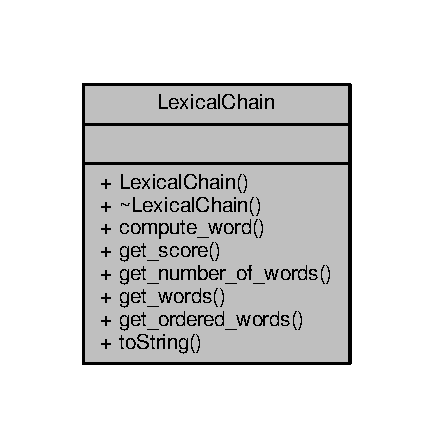
\includegraphics[width=208pt]{classLexicalChain__coll__graph}
\end{center}
\end{figure}
\subsection*{Public Member Functions}
\begin{DoxyCompactItemize}
\item 
\hyperlink{classLexicalChain_a1035313b140bb9833030d54f2a616082}{Lexical\+Chain} (\hyperlink{classRelation}{Relation} $\ast$r, const freeling\+::word \&w, const freeling\+::sentence \&s, int n\+\_\+paragraph, int n\+\_\+sentence, int position)
\begin{DoxyCompactList}\small\item\em Constructor. \end{DoxyCompactList}\item 
\hyperlink{classLexicalChain_a95f08ad98d07d5eec86cf68b77bc6eee}{$\sim$\+Lexical\+Chain} ()
\begin{DoxyCompactList}\small\item\em Destructor. \end{DoxyCompactList}\item 
bool \hyperlink{classLexicalChain_a22e252664430e855efd2adc05d120952}{compute\+\_\+word} (const freeling\+::word \&w, const freeling\+::sentence \&s, const freeling\+::document \&doc, int n\+\_\+paragraph, int n\+\_\+sentence, int position, std\+::wostream \&sout)
\begin{DoxyCompactList}\small\item\em Computes a word, if the word an be added to the lexical chain, this method stores it in its structures and return true. \end{DoxyCompactList}\item 
double \hyperlink{classLexicalChain_ad7b400e51350a05025d93ca1d97ee4a9}{get\+\_\+score} ()
\begin{DoxyCompactList}\small\item\em Get the score of the lexical chain. \end{DoxyCompactList}\item 
int \hyperlink{classLexicalChain_a43ccc424bcb3be5d7051853e0a310294}{get\+\_\+number\+\_\+of\+\_\+words} () const 
\begin{DoxyCompactList}\small\item\em Get the number of words inside the lexical chain. \end{DoxyCompactList}\item 
const std\+::list$<$ \hyperlink{structword__pos}{word\+\_\+pos} $>$ \& \hyperlink{classLexicalChain_ac3c54f9712f691928d1fb20d8924f441}{get\+\_\+words} () const 
\begin{DoxyCompactList}\small\item\em Get all the words embedded in a \hyperlink{structword__pos}{word\+\_\+pos} struct of the lexical chain. \end{DoxyCompactList}\item 
std\+::list$<$ \hyperlink{structword__pos}{word\+\_\+pos} $>$ \hyperlink{classLexicalChain_a64ab9f2876759a969c65e2dd098b621e}{get\+\_\+ordered\+\_\+words} () const 
\begin{DoxyCompactList}\small\item\em Get all the words ordered by frequency. \end{DoxyCompactList}\item 
std\+::wstring \hyperlink{classLexicalChain_ad5b4964c0dbee6e5376e7c350fc69962}{to\+String} ()
\begin{DoxyCompactList}\small\item\em Get a string representation of the lexical chain to debug. \end{DoxyCompactList}\end{DoxyCompactItemize}


\subsection{Detailed Description}
Class \hyperlink{classLexicalChain}{Lexical\+Chain} represents a lexical chain and computes words and stores (or not) them into the structures. 

\subsection{Constructor \& Destructor Documentation}
\hypertarget{classLexicalChain_a1035313b140bb9833030d54f2a616082}{}\index{Lexical\+Chain@{Lexical\+Chain}!Lexical\+Chain@{Lexical\+Chain}}
\index{Lexical\+Chain@{Lexical\+Chain}!Lexical\+Chain@{Lexical\+Chain}}
\subsubsection[{Lexical\+Chain}]{\setlength{\rightskip}{0pt plus 5cm}Lexical\+Chain\+::\+Lexical\+Chain (
\begin{DoxyParamCaption}
\item[{{\bf Relation} $\ast$}]{r, }
\item[{const freeling\+::word \&}]{w, }
\item[{const freeling\+::sentence \&}]{s, }
\item[{int}]{n\+\_\+paragraph, }
\item[{int}]{n\+\_\+sentence, }
\item[{int}]{position}
\end{DoxyParamCaption}
)}\label{classLexicalChain_a1035313b140bb9833030d54f2a616082}


Constructor. 

\hypertarget{classLexicalChain_a95f08ad98d07d5eec86cf68b77bc6eee}{}\index{Lexical\+Chain@{Lexical\+Chain}!````~Lexical\+Chain@{$\sim$\+Lexical\+Chain}}
\index{````~Lexical\+Chain@{$\sim$\+Lexical\+Chain}!Lexical\+Chain@{Lexical\+Chain}}
\subsubsection[{$\sim$\+Lexical\+Chain}]{\setlength{\rightskip}{0pt plus 5cm}Lexical\+Chain\+::$\sim$\+Lexical\+Chain (
\begin{DoxyParamCaption}
{}
\end{DoxyParamCaption}
)}\label{classLexicalChain_a95f08ad98d07d5eec86cf68b77bc6eee}


Destructor. 



\subsection{Member Function Documentation}
\hypertarget{classLexicalChain_a22e252664430e855efd2adc05d120952}{}\index{Lexical\+Chain@{Lexical\+Chain}!compute\+\_\+word@{compute\+\_\+word}}
\index{compute\+\_\+word@{compute\+\_\+word}!Lexical\+Chain@{Lexical\+Chain}}
\subsubsection[{compute\+\_\+word}]{\setlength{\rightskip}{0pt plus 5cm}bool Lexical\+Chain\+::compute\+\_\+word (
\begin{DoxyParamCaption}
\item[{const freeling\+::word \&}]{w, }
\item[{const freeling\+::sentence \&}]{s, }
\item[{const freeling\+::document \&}]{doc, }
\item[{int}]{n\+\_\+paragraph, }
\item[{int}]{n\+\_\+sentence, }
\item[{int}]{position, }
\item[{std\+::wostream \&}]{sout}
\end{DoxyParamCaption}
)}\label{classLexicalChain_a22e252664430e855efd2adc05d120952}


Computes a word, if the word an be added to the lexical chain, this method stores it in its structures and return true. 

Otherwise, it does nothing and returns false. \hypertarget{classLexicalChain_a43ccc424bcb3be5d7051853e0a310294}{}\index{Lexical\+Chain@{Lexical\+Chain}!get\+\_\+number\+\_\+of\+\_\+words@{get\+\_\+number\+\_\+of\+\_\+words}}
\index{get\+\_\+number\+\_\+of\+\_\+words@{get\+\_\+number\+\_\+of\+\_\+words}!Lexical\+Chain@{Lexical\+Chain}}
\subsubsection[{get\+\_\+number\+\_\+of\+\_\+words}]{\setlength{\rightskip}{0pt plus 5cm}int Lexical\+Chain\+::get\+\_\+number\+\_\+of\+\_\+words (
\begin{DoxyParamCaption}
{}
\end{DoxyParamCaption}
) const}\label{classLexicalChain_a43ccc424bcb3be5d7051853e0a310294}


Get the number of words inside the lexical chain. 

\hypertarget{classLexicalChain_a64ab9f2876759a969c65e2dd098b621e}{}\index{Lexical\+Chain@{Lexical\+Chain}!get\+\_\+ordered\+\_\+words@{get\+\_\+ordered\+\_\+words}}
\index{get\+\_\+ordered\+\_\+words@{get\+\_\+ordered\+\_\+words}!Lexical\+Chain@{Lexical\+Chain}}
\subsubsection[{get\+\_\+ordered\+\_\+words}]{\setlength{\rightskip}{0pt plus 5cm}list$<$ {\bf word\+\_\+pos} $>$ Lexical\+Chain\+::get\+\_\+ordered\+\_\+words (
\begin{DoxyParamCaption}
{}
\end{DoxyParamCaption}
) const}\label{classLexicalChain_a64ab9f2876759a969c65e2dd098b621e}


Get all the words ordered by frequency. 

\hypertarget{classLexicalChain_ad7b400e51350a05025d93ca1d97ee4a9}{}\index{Lexical\+Chain@{Lexical\+Chain}!get\+\_\+score@{get\+\_\+score}}
\index{get\+\_\+score@{get\+\_\+score}!Lexical\+Chain@{Lexical\+Chain}}
\subsubsection[{get\+\_\+score}]{\setlength{\rightskip}{0pt plus 5cm}double Lexical\+Chain\+::get\+\_\+score (
\begin{DoxyParamCaption}
{}
\end{DoxyParamCaption}
)}\label{classLexicalChain_ad7b400e51350a05025d93ca1d97ee4a9}


Get the score of the lexical chain. 

\hypertarget{classLexicalChain_ac3c54f9712f691928d1fb20d8924f441}{}\index{Lexical\+Chain@{Lexical\+Chain}!get\+\_\+words@{get\+\_\+words}}
\index{get\+\_\+words@{get\+\_\+words}!Lexical\+Chain@{Lexical\+Chain}}
\subsubsection[{get\+\_\+words}]{\setlength{\rightskip}{0pt plus 5cm}const list$<$ {\bf word\+\_\+pos} $>$ \& Lexical\+Chain\+::get\+\_\+words (
\begin{DoxyParamCaption}
{}
\end{DoxyParamCaption}
) const}\label{classLexicalChain_ac3c54f9712f691928d1fb20d8924f441}


Get all the words embedded in a \hyperlink{structword__pos}{word\+\_\+pos} struct of the lexical chain. 

\hypertarget{classLexicalChain_ad5b4964c0dbee6e5376e7c350fc69962}{}\index{Lexical\+Chain@{Lexical\+Chain}!to\+String@{to\+String}}
\index{to\+String@{to\+String}!Lexical\+Chain@{Lexical\+Chain}}
\subsubsection[{to\+String}]{\setlength{\rightskip}{0pt plus 5cm}wstring Lexical\+Chain\+::to\+String (
\begin{DoxyParamCaption}
{}
\end{DoxyParamCaption}
)}\label{classLexicalChain_ad5b4964c0dbee6e5376e7c350fc69962}


Get a string representation of the lexical chain to debug. 



The documentation for this class was generated from the following files\+:\begin{DoxyCompactItemize}
\item 
/home/samuel/\+Summarizer/src/\hyperlink{LexicalChain_8h}{Lexical\+Chain.\+h}\item 
/home/samuel/\+Summarizer/src/\hyperlink{LexicalChain_8cc}{Lexical\+Chain.\+cc}\end{DoxyCompactItemize}

\hypertarget{structrelated__words}{}\section{related\+\_\+words Struct Reference}
\label{structrelated__words}\index{related\+\_\+words@{related\+\_\+words}}


Struct that represents a relationship between two words.  




{\ttfamily \#include $<$Relation.\+h$>$}



Collaboration diagram for related\+\_\+words\+:
\nopagebreak
\begin{figure}[H]
\begin{center}
\leavevmode
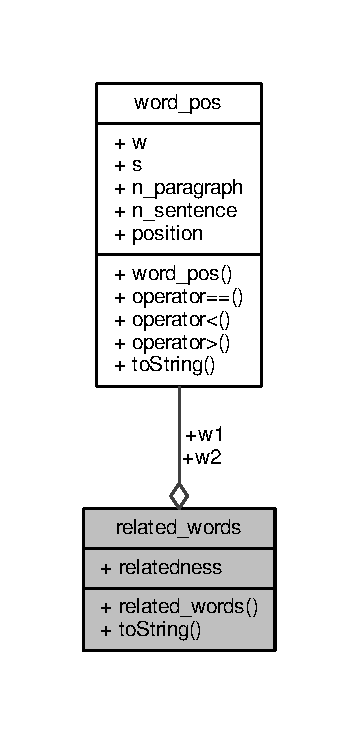
\includegraphics[width=172pt]{structrelated__words__coll__graph}
\end{center}
\end{figure}
\subsection*{Public Member Functions}
\begin{DoxyCompactItemize}
\item 
\hyperlink{structrelated__words_a0f35724f6fcc5cad5666b7b32c3cd36f}{related\+\_\+words} (const \hyperlink{structword__pos}{word\+\_\+pos} \&w\+\_\+p1, const \hyperlink{structword__pos}{word\+\_\+pos} \&w\+\_\+p2, double \hyperlink{structrelated__words_aefbff0c852fe59008f43f2c921b42330}{relatedness})
\item 
std\+::wstring \hyperlink{structrelated__words_a4feeb3a32b398b9b1f31197431bd0002}{to\+String} () const 
\begin{DoxyCompactList}\small\item\em Get a string representation of the relationship to debug. \end{DoxyCompactList}\end{DoxyCompactItemize}
\subsection*{Public Attributes}
\begin{DoxyCompactItemize}
\item 
const \hyperlink{structword__pos}{word\+\_\+pos} \& \hyperlink{structrelated__words_a442442bc95c4964a943f0d60c3a0eb30}{w1}
\item 
const \hyperlink{structword__pos}{word\+\_\+pos} \& \hyperlink{structrelated__words_a183d95179fe2892922bcd9485b48989f}{w2}
\item 
double \hyperlink{structrelated__words_aefbff0c852fe59008f43f2c921b42330}{relatedness}
\begin{DoxyCompactList}\small\item\em Relatedness represents the strength of the relationship. \end{DoxyCompactList}\end{DoxyCompactItemize}


\subsection{Detailed Description}
Struct that represents a relationship between two words. 

\subsection{Constructor \& Destructor Documentation}
\hypertarget{structrelated__words_a0f35724f6fcc5cad5666b7b32c3cd36f}{}\index{related\+\_\+words@{related\+\_\+words}!related\+\_\+words@{related\+\_\+words}}
\index{related\+\_\+words@{related\+\_\+words}!related\+\_\+words@{related\+\_\+words}}
\subsubsection[{related\+\_\+words}]{\setlength{\rightskip}{0pt plus 5cm}related\+\_\+words\+::related\+\_\+words (
\begin{DoxyParamCaption}
\item[{const {\bf word\+\_\+pos} \&}]{w\+\_\+p1, }
\item[{const {\bf word\+\_\+pos} \&}]{w\+\_\+p2, }
\item[{double}]{relatedness}
\end{DoxyParamCaption}
)}\label{structrelated__words_a0f35724f6fcc5cad5666b7b32c3cd36f}


\subsection{Member Function Documentation}
\hypertarget{structrelated__words_a4feeb3a32b398b9b1f31197431bd0002}{}\index{related\+\_\+words@{related\+\_\+words}!to\+String@{to\+String}}
\index{to\+String@{to\+String}!related\+\_\+words@{related\+\_\+words}}
\subsubsection[{to\+String}]{\setlength{\rightskip}{0pt plus 5cm}wstring related\+\_\+words\+::to\+String (
\begin{DoxyParamCaption}
{}
\end{DoxyParamCaption}
) const}\label{structrelated__words_a4feeb3a32b398b9b1f31197431bd0002}


Get a string representation of the relationship to debug. 



\subsection{Member Data Documentation}
\hypertarget{structrelated__words_aefbff0c852fe59008f43f2c921b42330}{}\index{related\+\_\+words@{related\+\_\+words}!relatedness@{relatedness}}
\index{relatedness@{relatedness}!related\+\_\+words@{related\+\_\+words}}
\subsubsection[{relatedness}]{\setlength{\rightskip}{0pt plus 5cm}double related\+\_\+words\+::relatedness}\label{structrelated__words_aefbff0c852fe59008f43f2c921b42330}


Relatedness represents the strength of the relationship. 

\hypertarget{structrelated__words_a442442bc95c4964a943f0d60c3a0eb30}{}\index{related\+\_\+words@{related\+\_\+words}!w1@{w1}}
\index{w1@{w1}!related\+\_\+words@{related\+\_\+words}}
\subsubsection[{w1}]{\setlength{\rightskip}{0pt plus 5cm}const {\bf word\+\_\+pos}\& related\+\_\+words\+::w1}\label{structrelated__words_a442442bc95c4964a943f0d60c3a0eb30}
\hypertarget{structrelated__words_a183d95179fe2892922bcd9485b48989f}{}\index{related\+\_\+words@{related\+\_\+words}!w2@{w2}}
\index{w2@{w2}!related\+\_\+words@{related\+\_\+words}}
\subsubsection[{w2}]{\setlength{\rightskip}{0pt plus 5cm}const {\bf word\+\_\+pos}\& related\+\_\+words\+::w2}\label{structrelated__words_a183d95179fe2892922bcd9485b48989f}


The documentation for this struct was generated from the following files\+:\begin{DoxyCompactItemize}
\item 
\hyperlink{Relation_8h}{Relation.\+h}\item 
\hyperlink{Relation_8cc}{Relation.\+cc}\end{DoxyCompactItemize}

\hypertarget{classRelation}{}\section{Relation Class Reference}
\label{classRelation}\index{Relation@{Relation}}


Class \hyperlink{classRelation}{Relation} is a non-\/instantiable class which defines many virtual methods to check if a word is compatible with the \hyperlink{classRelation}{Relation} or if a word can be stored in the structures of a lexical chain.  




{\ttfamily \#include $<$Relation.\+h$>$}



Inheritance diagram for Relation\+:\nopagebreak
\begin{figure}[H]
\begin{center}
\leavevmode
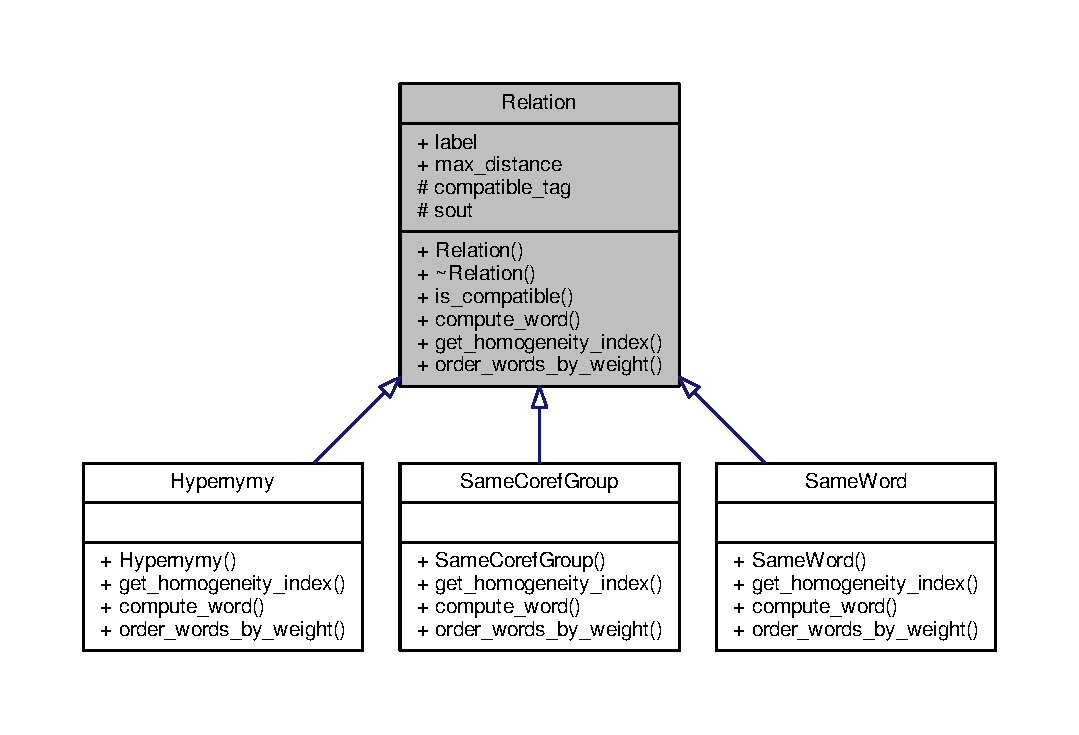
\includegraphics[width=350pt]{classRelation__inherit__graph}
\end{center}
\end{figure}


Collaboration diagram for Relation\+:\nopagebreak
\begin{figure}[H]
\begin{center}
\leavevmode
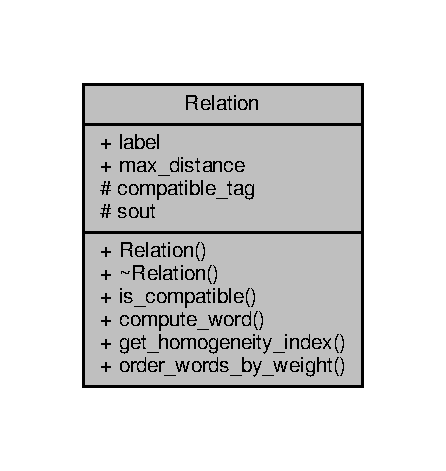
\includegraphics[width=214pt]{classRelation__coll__graph}
\end{center}
\end{figure}
\subsection*{Public Member Functions}
\begin{DoxyCompactItemize}
\item 
\hyperlink{classRelation_a4f4b35ad4cf4df6269634c9e4d5e4750}{Relation} (const std\+::wstring s, const std\+::wstring t)
\begin{DoxyCompactList}\small\item\em Constructor. \end{DoxyCompactList}\item 
\hyperlink{classRelation_ad8bc5c349f9d98b15972fd0b09f341cc}{$\sim$\+Relation} ()
\begin{DoxyCompactList}\small\item\em Destructor. \end{DoxyCompactList}\item 
bool \hyperlink{classRelation_a93391c4c61443f458b164b3732ee9584}{is\+\_\+compatible} (const freeling\+::word \&w) const 
\begin{DoxyCompactList}\small\item\em True if the words tag is compatible with the relation. \end{DoxyCompactList}\item 
virtual bool \hyperlink{classRelation_a977bc3e777d41eb53dcae0cd194d7a0b}{compute\+\_\+word} (const freeling\+::word \&w, const freeling\+::sentence \&s, const freeling\+::document \&doc, int n\+\_\+paragraph, int n\+\_\+sentence, int position, std\+::list$<$ \hyperlink{structword__pos}{word\+\_\+pos} $>$ \&words, std\+::list$<$ \hyperlink{structrelated__words}{related\+\_\+words} $>$ \&relations, std\+::unordered\+\_\+map$<$ std\+::wstring, std\+::pair$<$ int, \hyperlink{structword__pos}{word\+\_\+pos} $\ast$ $>$ $>$ \&unique\+\_\+words) const =0
\item 
virtual double \hyperlink{classRelation_a0037fb98b82d84643ad7f2e6c436d0a4}{get\+\_\+homogeneity\+\_\+index} (const std\+::list$<$ \hyperlink{structword__pos}{word\+\_\+pos} $>$ \&words, const std\+::list$<$ \hyperlink{structrelated__words}{related\+\_\+words} $>$ \&relations, const std\+::unordered\+\_\+map$<$ std\+::wstring, std\+::pair$<$ int, \hyperlink{structword__pos}{word\+\_\+pos} $\ast$ $>$ $>$ \&unique\+\_\+words)=0
\item 
virtual std\+::list$<$ \hyperlink{structword__pos}{word\+\_\+pos} $>$ \hyperlink{classRelation_ae19d8d190681b0f47a19d4fb0618b7b3}{order\+\_\+words\+\_\+by\+\_\+weight} (const std\+::unordered\+\_\+map$<$ std\+::wstring, std\+::pair$<$ int, \hyperlink{structword__pos}{word\+\_\+pos} $\ast$ $>$ $>$ \&unique\+\_\+words) const =0
\end{DoxyCompactItemize}
\subsection*{Public Attributes}
\begin{DoxyCompactItemize}
\item 
const std\+::wstring \hyperlink{classRelation_a4885622334809b177f87b9034d9218fe}{label}
\begin{DoxyCompactList}\small\item\em Label with the name of the related. It is used for debugging. \end{DoxyCompactList}\end{DoxyCompactItemize}
\subsection*{Static Public Attributes}
\begin{DoxyCompactItemize}
\item 
static int \hyperlink{classRelation_a634818cf4618e3862961d457e8ba0448}{max\+\_\+distance} = 0
\begin{DoxyCompactList}\small\item\em The maximum distance in phrases between two words to be related. \end{DoxyCompactList}\end{DoxyCompactItemize}
\subsection*{Protected Attributes}
\begin{DoxyCompactItemize}
\item 
const freeling\+::regexp \hyperlink{classRelation_a3c44dc364bd5530017a4828fee9a14bf}{compatible\+\_\+tag}
\begin{DoxyCompactList}\small\item\em If a word tag matchs with compatible\+\_\+tag, then the word is compatible with the relation. \end{DoxyCompactList}\item 
std\+::wostream $\ast$ \hyperlink{classRelation_a44deec0ee05d803ea23e14520fd57a75}{sout}
\begin{DoxyCompactList}\small\item\em Pointer to a wostream to debug. \end{DoxyCompactList}\end{DoxyCompactItemize}


\subsection{Detailed Description}
Class \hyperlink{classRelation}{Relation} is a non-\/instantiable class which defines many virtual methods to check if a word is compatible with the \hyperlink{classRelation}{Relation} or if a word can be stored in the structures of a lexical chain. 

\subsection{Constructor \& Destructor Documentation}
\hypertarget{classRelation_a4f4b35ad4cf4df6269634c9e4d5e4750}{}\index{Relation@{Relation}!Relation@{Relation}}
\index{Relation@{Relation}!Relation@{Relation}}
\subsubsection[{Relation}]{\setlength{\rightskip}{0pt plus 5cm}Relation\+::\+Relation (
\begin{DoxyParamCaption}
\item[{const std\+::wstring}]{s, }
\item[{const std\+::wstring}]{t}
\end{DoxyParamCaption}
)}\label{classRelation_a4f4b35ad4cf4df6269634c9e4d5e4750}


Constructor. 

\hypertarget{classRelation_ad8bc5c349f9d98b15972fd0b09f341cc}{}\index{Relation@{Relation}!````~Relation@{$\sim$\+Relation}}
\index{````~Relation@{$\sim$\+Relation}!Relation@{Relation}}
\subsubsection[{$\sim$\+Relation}]{\setlength{\rightskip}{0pt plus 5cm}Relation\+::$\sim$\+Relation (
\begin{DoxyParamCaption}
{}
\end{DoxyParamCaption}
)}\label{classRelation_ad8bc5c349f9d98b15972fd0b09f341cc}


Destructor. 



\subsection{Member Function Documentation}
\hypertarget{classRelation_a977bc3e777d41eb53dcae0cd194d7a0b}{}\index{Relation@{Relation}!compute\+\_\+word@{compute\+\_\+word}}
\index{compute\+\_\+word@{compute\+\_\+word}!Relation@{Relation}}
\subsubsection[{compute\+\_\+word}]{\setlength{\rightskip}{0pt plus 5cm}bool Relation\+::compute\+\_\+word (
\begin{DoxyParamCaption}
\item[{const freeling\+::word \&}]{w, }
\item[{const freeling\+::sentence \&}]{s, }
\item[{const freeling\+::document \&}]{doc, }
\item[{int}]{n\+\_\+paragraph, }
\item[{int}]{n\+\_\+sentence, }
\item[{int}]{position, }
\item[{std\+::list$<$ {\bf word\+\_\+pos} $>$ \&}]{words, }
\item[{std\+::list$<$ {\bf related\+\_\+words} $>$ \&}]{relations, }
\item[{std\+::unordered\+\_\+map$<$ std\+::wstring, std\+::pair$<$ int, {\bf word\+\_\+pos} $\ast$ $>$ $>$ \&}]{unique\+\_\+words}
\end{DoxyParamCaption}
) const\hspace{0.3cm}{\ttfamily [pure virtual]}}\label{classRelation_a977bc3e777d41eb53dcae0cd194d7a0b}


Implemented in \hyperlink{classSameCorefGroup_a6e2b2784fbac185dc16af242280ff082}{Same\+Coref\+Group}, \hyperlink{classHypernymy_a9eb6e16f7b8128b9865c43df41940a77}{Hypernymy}, and \hyperlink{classSameWord_a3773253aec894b3a50c5d03e5725f4bf}{Same\+Word}.

\hypertarget{classRelation_a0037fb98b82d84643ad7f2e6c436d0a4}{}\index{Relation@{Relation}!get\+\_\+homogeneity\+\_\+index@{get\+\_\+homogeneity\+\_\+index}}
\index{get\+\_\+homogeneity\+\_\+index@{get\+\_\+homogeneity\+\_\+index}!Relation@{Relation}}
\subsubsection[{get\+\_\+homogeneity\+\_\+index}]{\setlength{\rightskip}{0pt plus 5cm}virtual double Relation\+::get\+\_\+homogeneity\+\_\+index (
\begin{DoxyParamCaption}
\item[{const std\+::list$<$ {\bf word\+\_\+pos} $>$ \&}]{words, }
\item[{const std\+::list$<$ {\bf related\+\_\+words} $>$ \&}]{relations, }
\item[{const std\+::unordered\+\_\+map$<$ std\+::wstring, std\+::pair$<$ int, {\bf word\+\_\+pos} $\ast$ $>$ $>$ \&}]{unique\+\_\+words}
\end{DoxyParamCaption}
)\hspace{0.3cm}{\ttfamily [pure virtual]}}\label{classRelation_a0037fb98b82d84643ad7f2e6c436d0a4}


Implemented in \hyperlink{classSameCorefGroup_a7b6e236b68a30f2b24e5838af6c16a7b}{Same\+Coref\+Group}, \hyperlink{classHypernymy_a597074abd7795e114d13783677e55e20}{Hypernymy}, and \hyperlink{classSameWord_a3c0506fe869c16d2c7d20d5647a6c99f}{Same\+Word}.

\hypertarget{classRelation_a93391c4c61443f458b164b3732ee9584}{}\index{Relation@{Relation}!is\+\_\+compatible@{is\+\_\+compatible}}
\index{is\+\_\+compatible@{is\+\_\+compatible}!Relation@{Relation}}
\subsubsection[{is\+\_\+compatible}]{\setlength{\rightskip}{0pt plus 5cm}bool Relation\+::is\+\_\+compatible (
\begin{DoxyParamCaption}
\item[{const freeling\+::word \&}]{w}
\end{DoxyParamCaption}
) const}\label{classRelation_a93391c4c61443f458b164b3732ee9584}


True if the words tag is compatible with the relation. 

\hypertarget{classRelation_ae19d8d190681b0f47a19d4fb0618b7b3}{}\index{Relation@{Relation}!order\+\_\+words\+\_\+by\+\_\+weight@{order\+\_\+words\+\_\+by\+\_\+weight}}
\index{order\+\_\+words\+\_\+by\+\_\+weight@{order\+\_\+words\+\_\+by\+\_\+weight}!Relation@{Relation}}
\subsubsection[{order\+\_\+words\+\_\+by\+\_\+weight}]{\setlength{\rightskip}{0pt plus 5cm}virtual std\+::list$<${\bf word\+\_\+pos}$>$ Relation\+::order\+\_\+words\+\_\+by\+\_\+weight (
\begin{DoxyParamCaption}
\item[{const std\+::unordered\+\_\+map$<$ std\+::wstring, std\+::pair$<$ int, {\bf word\+\_\+pos} $\ast$ $>$ $>$ \&}]{unique\+\_\+words}
\end{DoxyParamCaption}
) const\hspace{0.3cm}{\ttfamily [pure virtual]}}\label{classRelation_ae19d8d190681b0f47a19d4fb0618b7b3}


Implemented in \hyperlink{classSameCorefGroup_a44e442d53523999350cbb37cb40918f4}{Same\+Coref\+Group}, \hyperlink{classHypernymy_aaa6ac1db9e77a937d38f6e19c550f62f}{Hypernymy}, and \hyperlink{classSameWord_a633fbd80c1abe38b71af82cc3fb3e528}{Same\+Word}.



\subsection{Member Data Documentation}
\hypertarget{classRelation_a3c44dc364bd5530017a4828fee9a14bf}{}\index{Relation@{Relation}!compatible\+\_\+tag@{compatible\+\_\+tag}}
\index{compatible\+\_\+tag@{compatible\+\_\+tag}!Relation@{Relation}}
\subsubsection[{compatible\+\_\+tag}]{\setlength{\rightskip}{0pt plus 5cm}const freeling\+::regexp Relation\+::compatible\+\_\+tag\hspace{0.3cm}{\ttfamily [protected]}}\label{classRelation_a3c44dc364bd5530017a4828fee9a14bf}


If a word tag matchs with compatible\+\_\+tag, then the word is compatible with the relation. 

\hypertarget{classRelation_a4885622334809b177f87b9034d9218fe}{}\index{Relation@{Relation}!label@{label}}
\index{label@{label}!Relation@{Relation}}
\subsubsection[{label}]{\setlength{\rightskip}{0pt plus 5cm}const std\+::wstring Relation\+::label}\label{classRelation_a4885622334809b177f87b9034d9218fe}


Label with the name of the related. It is used for debugging. 

\hypertarget{classRelation_a634818cf4618e3862961d457e8ba0448}{}\index{Relation@{Relation}!max\+\_\+distance@{max\+\_\+distance}}
\index{max\+\_\+distance@{max\+\_\+distance}!Relation@{Relation}}
\subsubsection[{max\+\_\+distance}]{\setlength{\rightskip}{0pt plus 5cm}int Relation\+::max\+\_\+distance = 0\hspace{0.3cm}{\ttfamily [static]}}\label{classRelation_a634818cf4618e3862961d457e8ba0448}


The maximum distance in phrases between two words to be related. 

\hypertarget{classRelation_a44deec0ee05d803ea23e14520fd57a75}{}\index{Relation@{Relation}!sout@{sout}}
\index{sout@{sout}!Relation@{Relation}}
\subsubsection[{sout}]{\setlength{\rightskip}{0pt plus 5cm}std\+::wostream$\ast$ Relation\+::sout\hspace{0.3cm}{\ttfamily [protected]}}\label{classRelation_a44deec0ee05d803ea23e14520fd57a75}


Pointer to a wostream to debug. 



The documentation for this class was generated from the following files\+:\begin{DoxyCompactItemize}
\item 
\hyperlink{Relation_8h}{Relation.\+h}\item 
\hyperlink{Relation_8cc}{Relation.\+cc}\end{DoxyCompactItemize}

\hypertarget{classSameCorefGroup}{}\section{Same\+Coref\+Group Class Reference}
\label{classSameCorefGroup}\index{Same\+Coref\+Group@{Same\+Coref\+Group}}


Class \hyperlink{classSameCorefGroup}{Same\+Coref\+Group} represents the same coreference group relation\+: two words are related if they are in the same coreference group.  




{\ttfamily \#include $<$Relation.\+h$>$}



Inheritance diagram for Same\+Coref\+Group\+:
\nopagebreak
\begin{figure}[H]
\begin{center}
\leavevmode
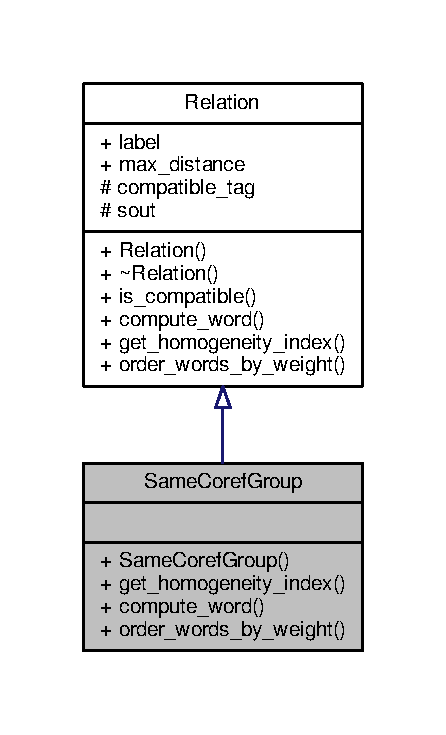
\includegraphics[width=214pt]{classSameCorefGroup__inherit__graph}
\end{center}
\end{figure}


Collaboration diagram for Same\+Coref\+Group\+:
\nopagebreak
\begin{figure}[H]
\begin{center}
\leavevmode
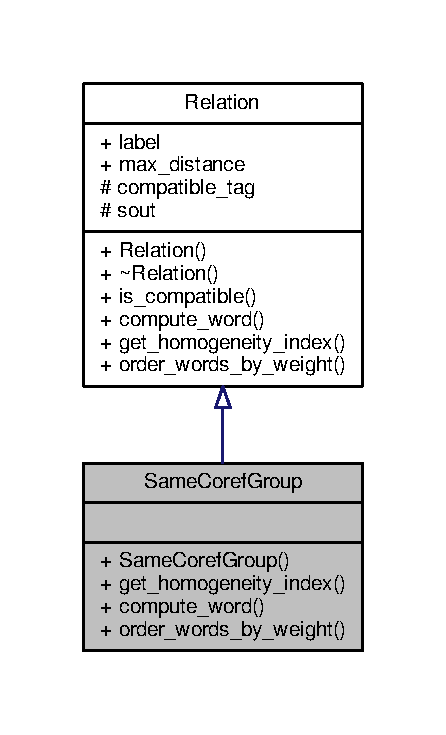
\includegraphics[width=214pt]{classSameCorefGroup__coll__graph}
\end{center}
\end{figure}
\subsection*{Public Member Functions}
\begin{DoxyCompactItemize}
\item 
\hyperlink{classSameCorefGroup_aa38679729573a9800ecbaa1650ca2458}{Same\+Coref\+Group} (std\+::wostream \&\hyperlink{classRelation_a44deec0ee05d803ea23e14520fd57a75}{sout})
\begin{DoxyCompactList}\small\item\em Constructor. \end{DoxyCompactList}\item 
double \hyperlink{classSameCorefGroup_a7b6e236b68a30f2b24e5838af6c16a7b}{get\+\_\+homogeneity\+\_\+index} (const std\+::list$<$ \hyperlink{structword__pos}{word\+\_\+pos} $>$ \&words, const std\+::list$<$ \hyperlink{structrelated__words}{related\+\_\+words} $>$ \&relations, const std\+::unordered\+\_\+map$<$ std\+::wstring, std\+::pair$<$ int, \hyperlink{structword__pos}{word\+\_\+pos} $\ast$ $>$ $>$ \&unique\+\_\+words)
\begin{DoxyCompactList}\small\item\em Computes the homogeinity index of the given structures using the specific formula of this relation. \end{DoxyCompactList}\item 
bool \hyperlink{classSameCorefGroup_a6e2b2784fbac185dc16af242280ff082}{compute\+\_\+word} (const freeling\+::word \&w, const freeling\+::sentence \&s, const freeling\+::document \&doc, int n\+\_\+paragraph, int n\+\_\+sentence, int position, std\+::list$<$ \hyperlink{structword__pos}{word\+\_\+pos} $>$ \&words, std\+::list$<$ \hyperlink{structrelated__words}{related\+\_\+words} $>$ \&relations, std\+::unordered\+\_\+map$<$ std\+::wstring, std\+::pair$<$ int, \hyperlink{structword__pos}{word\+\_\+pos} $\ast$ $>$ $>$ \&unique\+\_\+words) const 
\begin{DoxyCompactList}\small\item\em Returns true and stores the word w in the list words, list relations and unordered\+\_\+map unique\+\_\+words if w is compatible with the words in these structures using this relation. \end{DoxyCompactList}\item 
std\+::list$<$ \hyperlink{structword__pos}{word\+\_\+pos} $>$ \hyperlink{classSameCorefGroup_a44e442d53523999350cbb37cb40918f4}{order\+\_\+words\+\_\+by\+\_\+weight} (const std\+::unordered\+\_\+map$<$ std\+::wstring, std\+::pair$<$ int, \hyperlink{structword__pos}{word\+\_\+pos} $\ast$ $>$ $>$ \&unique\+\_\+words) const 
\begin{DoxyCompactList}\small\item\em Sorts the words in unique\+\_\+words by word frequency and returns a list with them. \end{DoxyCompactList}\end{DoxyCompactItemize}
\subsection*{Additional Inherited Members}


\subsection{Detailed Description}
Class \hyperlink{classSameCorefGroup}{Same\+Coref\+Group} represents the same coreference group relation\+: two words are related if they are in the same coreference group. 

\subsection{Constructor \& Destructor Documentation}
\hypertarget{classSameCorefGroup_aa38679729573a9800ecbaa1650ca2458}{}\index{Same\+Coref\+Group@{Same\+Coref\+Group}!Same\+Coref\+Group@{Same\+Coref\+Group}}
\index{Same\+Coref\+Group@{Same\+Coref\+Group}!Same\+Coref\+Group@{Same\+Coref\+Group}}
\subsubsection[{Same\+Coref\+Group}]{\setlength{\rightskip}{0pt plus 5cm}Same\+Coref\+Group\+::\+Same\+Coref\+Group (
\begin{DoxyParamCaption}
\item[{std\+::wostream \&}]{sout}
\end{DoxyParamCaption}
)}\label{classSameCorefGroup_aa38679729573a9800ecbaa1650ca2458}


Constructor. 



\subsection{Member Function Documentation}
\hypertarget{classSameCorefGroup_a6e2b2784fbac185dc16af242280ff082}{}\index{Same\+Coref\+Group@{Same\+Coref\+Group}!compute\+\_\+word@{compute\+\_\+word}}
\index{compute\+\_\+word@{compute\+\_\+word}!Same\+Coref\+Group@{Same\+Coref\+Group}}
\subsubsection[{compute\+\_\+word}]{\setlength{\rightskip}{0pt plus 5cm}bool Same\+Coref\+Group\+::compute\+\_\+word (
\begin{DoxyParamCaption}
\item[{const freeling\+::word \&}]{w, }
\item[{const freeling\+::sentence \&}]{s, }
\item[{const freeling\+::document \&}]{doc, }
\item[{int}]{n\+\_\+paragraph, }
\item[{int}]{n\+\_\+sentence, }
\item[{int}]{position, }
\item[{std\+::list$<$ {\bf word\+\_\+pos} $>$ \&}]{words, }
\item[{std\+::list$<$ {\bf related\+\_\+words} $>$ \&}]{relations, }
\item[{std\+::unordered\+\_\+map$<$ std\+::wstring, std\+::pair$<$ int, {\bf word\+\_\+pos} $\ast$ $>$ $>$ \&}]{unique\+\_\+words}
\end{DoxyParamCaption}
) const\hspace{0.3cm}{\ttfamily [virtual]}}\label{classSameCorefGroup_a6e2b2784fbac185dc16af242280ff082}


Returns true and stores the word w in the list words, list relations and unordered\+\_\+map unique\+\_\+words if w is compatible with the words in these structures using this relation. 



Implements \hyperlink{classRelation_a977bc3e777d41eb53dcae0cd194d7a0b}{Relation}.

\hypertarget{classSameCorefGroup_a7b6e236b68a30f2b24e5838af6c16a7b}{}\index{Same\+Coref\+Group@{Same\+Coref\+Group}!get\+\_\+homogeneity\+\_\+index@{get\+\_\+homogeneity\+\_\+index}}
\index{get\+\_\+homogeneity\+\_\+index@{get\+\_\+homogeneity\+\_\+index}!Same\+Coref\+Group@{Same\+Coref\+Group}}
\subsubsection[{get\+\_\+homogeneity\+\_\+index}]{\setlength{\rightskip}{0pt plus 5cm}double Same\+Coref\+Group\+::get\+\_\+homogeneity\+\_\+index (
\begin{DoxyParamCaption}
\item[{const std\+::list$<$ {\bf word\+\_\+pos} $>$ \&}]{words, }
\item[{const std\+::list$<$ {\bf related\+\_\+words} $>$ \&}]{relations, }
\item[{const std\+::unordered\+\_\+map$<$ std\+::wstring, std\+::pair$<$ int, {\bf word\+\_\+pos} $\ast$ $>$ $>$ \&}]{unique\+\_\+words}
\end{DoxyParamCaption}
)\hspace{0.3cm}{\ttfamily [virtual]}}\label{classSameCorefGroup_a7b6e236b68a30f2b24e5838af6c16a7b}


Computes the homogeinity index of the given structures using the specific formula of this relation. 



Implements \hyperlink{classRelation_a0037fb98b82d84643ad7f2e6c436d0a4}{Relation}.

\hypertarget{classSameCorefGroup_a44e442d53523999350cbb37cb40918f4}{}\index{Same\+Coref\+Group@{Same\+Coref\+Group}!order\+\_\+words\+\_\+by\+\_\+weight@{order\+\_\+words\+\_\+by\+\_\+weight}}
\index{order\+\_\+words\+\_\+by\+\_\+weight@{order\+\_\+words\+\_\+by\+\_\+weight}!Same\+Coref\+Group@{Same\+Coref\+Group}}
\subsubsection[{order\+\_\+words\+\_\+by\+\_\+weight}]{\setlength{\rightskip}{0pt plus 5cm}list$<$ {\bf word\+\_\+pos} $>$ Same\+Coref\+Group\+::order\+\_\+words\+\_\+by\+\_\+weight (
\begin{DoxyParamCaption}
\item[{const std\+::unordered\+\_\+map$<$ std\+::wstring, std\+::pair$<$ int, {\bf word\+\_\+pos} $\ast$ $>$ $>$ \&}]{unique\+\_\+words}
\end{DoxyParamCaption}
) const\hspace{0.3cm}{\ttfamily [virtual]}}\label{classSameCorefGroup_a44e442d53523999350cbb37cb40918f4}


Sorts the words in unique\+\_\+words by word frequency and returns a list with them. 



Implements \hyperlink{classRelation_ae19d8d190681b0f47a19d4fb0618b7b3}{Relation}.



The documentation for this class was generated from the following files\+:\begin{DoxyCompactItemize}
\item 
\hyperlink{Relation_8h}{Relation.\+h}\item 
\hyperlink{Relation_8cc}{Relation.\+cc}\end{DoxyCompactItemize}

\hypertarget{classSameWord}{}\section{Same\+Word Class Reference}
\label{classSameWord}\index{Same\+Word@{Same\+Word}}


Class \hyperlink{classSameWord}{Same\+Word} represents the same word relation\+: two words are related if they are the same word.  




{\ttfamily \#include $<$Relation.\+h$>$}



Inheritance diagram for Same\+Word\+:
\nopagebreak
\begin{figure}[H]
\begin{center}
\leavevmode
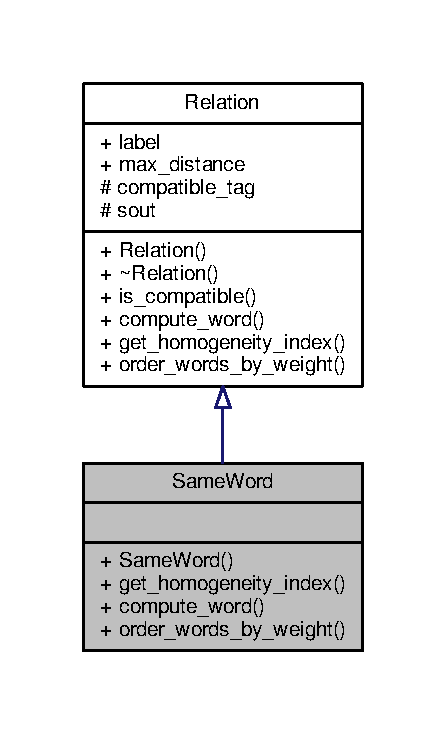
\includegraphics[width=214pt]{classSameWord__inherit__graph}
\end{center}
\end{figure}


Collaboration diagram for Same\+Word\+:
\nopagebreak
\begin{figure}[H]
\begin{center}
\leavevmode
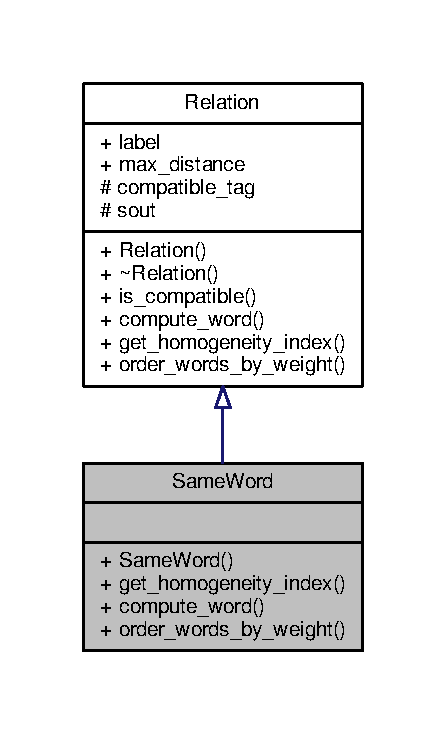
\includegraphics[width=214pt]{classSameWord__coll__graph}
\end{center}
\end{figure}
\subsection*{Public Member Functions}
\begin{DoxyCompactItemize}
\item 
\hyperlink{classSameWord_ac0dd07d610c7e8493ddaaf17c00db078}{Same\+Word} (std\+::wostream \&\hyperlink{classRelation_a44deec0ee05d803ea23e14520fd57a75}{sout})
\begin{DoxyCompactList}\small\item\em Constructor. \end{DoxyCompactList}\item 
double \hyperlink{classSameWord_a3c0506fe869c16d2c7d20d5647a6c99f}{get\+\_\+homogeneity\+\_\+index} (const std\+::list$<$ \hyperlink{structword__pos}{word\+\_\+pos} $>$ \&words, const std\+::list$<$ \hyperlink{structrelated__words}{related\+\_\+words} $>$ \&relations, const std\+::unordered\+\_\+map$<$ std\+::wstring, std\+::pair$<$ int, \hyperlink{structword__pos}{word\+\_\+pos} $\ast$ $>$ $>$ \&unique\+\_\+words)
\begin{DoxyCompactList}\small\item\em Computes the homogeinity index of the given structures using the specific formula of this relation. \end{DoxyCompactList}\item 
bool \hyperlink{classSameWord_a3773253aec894b3a50c5d03e5725f4bf}{compute\+\_\+word} (const freeling\+::word \&w, const freeling\+::sentence \&s, const freeling\+::document \&doc, int n\+\_\+paragraph, int n\+\_\+sentence, int position, std\+::list$<$ \hyperlink{structword__pos}{word\+\_\+pos} $>$ \&words, std\+::list$<$ \hyperlink{structrelated__words}{related\+\_\+words} $>$ \&relations, std\+::unordered\+\_\+map$<$ std\+::wstring, std\+::pair$<$ int, \hyperlink{structword__pos}{word\+\_\+pos} $\ast$ $>$ $>$ \&unique\+\_\+words) const 
\begin{DoxyCompactList}\small\item\em Returns true and stores the word w in the list words, list relations and unordered\+\_\+map unique\+\_\+words if w is compatible with the words in these structures using this relation. \end{DoxyCompactList}\item 
std\+::list$<$ \hyperlink{structword__pos}{word\+\_\+pos} $>$ \hyperlink{classSameWord_a633fbd80c1abe38b71af82cc3fb3e528}{order\+\_\+words\+\_\+by\+\_\+weight} (const std\+::unordered\+\_\+map$<$ std\+::wstring, std\+::pair$<$ int, \hyperlink{structword__pos}{word\+\_\+pos} $\ast$ $>$ $>$ \&unique\+\_\+words) const 
\begin{DoxyCompactList}\small\item\em In \hyperlink{classSameWord}{Same\+Word}, the words in unique\+\_\+words are not sorted because there is just one word. \end{DoxyCompactList}\end{DoxyCompactItemize}
\subsection*{Additional Inherited Members}


\subsection{Detailed Description}
Class \hyperlink{classSameWord}{Same\+Word} represents the same word relation\+: two words are related if they are the same word. 

\subsection{Constructor \& Destructor Documentation}
\hypertarget{classSameWord_ac0dd07d610c7e8493ddaaf17c00db078}{}\index{Same\+Word@{Same\+Word}!Same\+Word@{Same\+Word}}
\index{Same\+Word@{Same\+Word}!Same\+Word@{Same\+Word}}
\subsubsection[{Same\+Word}]{\setlength{\rightskip}{0pt plus 5cm}Same\+Word\+::\+Same\+Word (
\begin{DoxyParamCaption}
\item[{std\+::wostream \&}]{sout}
\end{DoxyParamCaption}
)}\label{classSameWord_ac0dd07d610c7e8493ddaaf17c00db078}


Constructor. 



\subsection{Member Function Documentation}
\hypertarget{classSameWord_a3773253aec894b3a50c5d03e5725f4bf}{}\index{Same\+Word@{Same\+Word}!compute\+\_\+word@{compute\+\_\+word}}
\index{compute\+\_\+word@{compute\+\_\+word}!Same\+Word@{Same\+Word}}
\subsubsection[{compute\+\_\+word}]{\setlength{\rightskip}{0pt plus 5cm}bool Same\+Word\+::compute\+\_\+word (
\begin{DoxyParamCaption}
\item[{const freeling\+::word \&}]{w, }
\item[{const freeling\+::sentence \&}]{s, }
\item[{const freeling\+::document \&}]{doc, }
\item[{int}]{n\+\_\+paragraph, }
\item[{int}]{n\+\_\+sentence, }
\item[{int}]{position, }
\item[{std\+::list$<$ {\bf word\+\_\+pos} $>$ \&}]{words, }
\item[{std\+::list$<$ {\bf related\+\_\+words} $>$ \&}]{relations, }
\item[{std\+::unordered\+\_\+map$<$ std\+::wstring, std\+::pair$<$ int, {\bf word\+\_\+pos} $\ast$ $>$ $>$ \&}]{unique\+\_\+words}
\end{DoxyParamCaption}
) const\hspace{0.3cm}{\ttfamily [virtual]}}\label{classSameWord_a3773253aec894b3a50c5d03e5725f4bf}


Returns true and stores the word w in the list words, list relations and unordered\+\_\+map unique\+\_\+words if w is compatible with the words in these structures using this relation. 



Implements \hyperlink{classRelation_a977bc3e777d41eb53dcae0cd194d7a0b}{Relation}.

\hypertarget{classSameWord_a3c0506fe869c16d2c7d20d5647a6c99f}{}\index{Same\+Word@{Same\+Word}!get\+\_\+homogeneity\+\_\+index@{get\+\_\+homogeneity\+\_\+index}}
\index{get\+\_\+homogeneity\+\_\+index@{get\+\_\+homogeneity\+\_\+index}!Same\+Word@{Same\+Word}}
\subsubsection[{get\+\_\+homogeneity\+\_\+index}]{\setlength{\rightskip}{0pt plus 5cm}double Same\+Word\+::get\+\_\+homogeneity\+\_\+index (
\begin{DoxyParamCaption}
\item[{const std\+::list$<$ {\bf word\+\_\+pos} $>$ \&}]{words, }
\item[{const std\+::list$<$ {\bf related\+\_\+words} $>$ \&}]{relations, }
\item[{const std\+::unordered\+\_\+map$<$ std\+::wstring, std\+::pair$<$ int, {\bf word\+\_\+pos} $\ast$ $>$ $>$ \&}]{unique\+\_\+words}
\end{DoxyParamCaption}
)\hspace{0.3cm}{\ttfamily [virtual]}}\label{classSameWord_a3c0506fe869c16d2c7d20d5647a6c99f}


Computes the homogeinity index of the given structures using the specific formula of this relation. 



Implements \hyperlink{classRelation_a0037fb98b82d84643ad7f2e6c436d0a4}{Relation}.

\hypertarget{classSameWord_a633fbd80c1abe38b71af82cc3fb3e528}{}\index{Same\+Word@{Same\+Word}!order\+\_\+words\+\_\+by\+\_\+weight@{order\+\_\+words\+\_\+by\+\_\+weight}}
\index{order\+\_\+words\+\_\+by\+\_\+weight@{order\+\_\+words\+\_\+by\+\_\+weight}!Same\+Word@{Same\+Word}}
\subsubsection[{order\+\_\+words\+\_\+by\+\_\+weight}]{\setlength{\rightskip}{0pt plus 5cm}list$<$ {\bf word\+\_\+pos} $>$ Same\+Word\+::order\+\_\+words\+\_\+by\+\_\+weight (
\begin{DoxyParamCaption}
\item[{const std\+::unordered\+\_\+map$<$ std\+::wstring, std\+::pair$<$ int, {\bf word\+\_\+pos} $\ast$ $>$ $>$ \&}]{unique\+\_\+words}
\end{DoxyParamCaption}
) const\hspace{0.3cm}{\ttfamily [virtual]}}\label{classSameWord_a633fbd80c1abe38b71af82cc3fb3e528}


In \hyperlink{classSameWord}{Same\+Word}, the words in unique\+\_\+words are not sorted because there is just one word. 

It returns the \hyperlink{structword__pos}{word\+\_\+pos} in unique\+\_\+words in a list. 

Implements \hyperlink{classRelation_ae19d8d190681b0f47a19d4fb0618b7b3}{Relation}.



The documentation for this class was generated from the following files\+:\begin{DoxyCompactItemize}
\item 
\hyperlink{Relation_8h}{Relation.\+h}\item 
\hyperlink{Relation_8cc}{Relation.\+cc}\end{DoxyCompactItemize}

\hypertarget{classSummarizer}{}\section{Summarizer Class Reference}
\label{classSummarizer}\index{Summarizer@{Summarizer}}


\hyperlink{classSummarizer}{Summarizer} class summarizes a document using the lexical chains method.  




{\ttfamily \#include $<$Summarizer.\+h$>$}



Collaboration diagram for Summarizer\+:\nopagebreak
\begin{figure}[H]
\begin{center}
\leavevmode
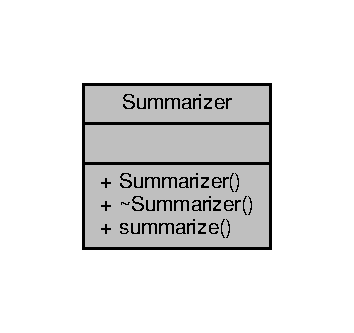
\includegraphics[width=170pt]{classSummarizer__coll__graph}
\end{center}
\end{figure}
\subsection*{Public Member Functions}
\begin{DoxyCompactItemize}
\item 
\hyperlink{classSummarizer_ae24d5afc2f3c61a287379e2b614726ac}{Summarizer} (const std\+::wstring \&dat\+File, bool debug)
\begin{DoxyCompactList}\small\item\em Constructor. \end{DoxyCompactList}\item 
\hyperlink{classSummarizer_a787d7b2274aeb313acd19d150437d4f5}{$\sim$\+Summarizer} ()
\begin{DoxyCompactList}\small\item\em Destructor. \end{DoxyCompactList}\item 
std\+::list$<$ const freeling\+::sentence $\ast$ $>$ \hyperlink{classSummarizer_a70a36036e96b1b03175c3f1fdde9d0e1}{summarize} (std\+::wostream \&sout, const freeling\+::document \&doc)
\begin{DoxyCompactList}\small\item\em Summarizes a document and returns the list of sentences that composes the summary. \end{DoxyCompactList}\end{DoxyCompactItemize}


\subsection{Detailed Description}
\hyperlink{classSummarizer}{Summarizer} class summarizes a document using the lexical chains method. 

\subsection{Constructor \& Destructor Documentation}
\hypertarget{classSummarizer_ae24d5afc2f3c61a287379e2b614726ac}{}\index{Summarizer@{Summarizer}!Summarizer@{Summarizer}}
\index{Summarizer@{Summarizer}!Summarizer@{Summarizer}}
\subsubsection[{Summarizer}]{\setlength{\rightskip}{0pt plus 5cm}Summarizer\+::\+Summarizer (
\begin{DoxyParamCaption}
\item[{const std\+::wstring \&}]{dat\+File, }
\item[{bool}]{debug}
\end{DoxyParamCaption}
)}\label{classSummarizer_ae24d5afc2f3c61a287379e2b614726ac}


Constructor. 

\hypertarget{classSummarizer_a787d7b2274aeb313acd19d150437d4f5}{}\index{Summarizer@{Summarizer}!````~Summarizer@{$\sim$\+Summarizer}}
\index{````~Summarizer@{$\sim$\+Summarizer}!Summarizer@{Summarizer}}
\subsubsection[{$\sim$\+Summarizer}]{\setlength{\rightskip}{0pt plus 5cm}Summarizer\+::$\sim$\+Summarizer (
\begin{DoxyParamCaption}
{}
\end{DoxyParamCaption}
)}\label{classSummarizer_a787d7b2274aeb313acd19d150437d4f5}


Destructor. 



\subsection{Member Function Documentation}
\hypertarget{classSummarizer_a70a36036e96b1b03175c3f1fdde9d0e1}{}\index{Summarizer@{Summarizer}!summarize@{summarize}}
\index{summarize@{summarize}!Summarizer@{Summarizer}}
\subsubsection[{summarize}]{\setlength{\rightskip}{0pt plus 5cm}list$<$ const sentence $\ast$ $>$ Summarizer\+::summarize (
\begin{DoxyParamCaption}
\item[{std\+::wostream \&}]{sout, }
\item[{const freeling\+::document \&}]{doc}
\end{DoxyParamCaption}
)}\label{classSummarizer_a70a36036e96b1b03175c3f1fdde9d0e1}


Summarizes a document and returns the list of sentences that composes the summary. 



The documentation for this class was generated from the following files\+:\begin{DoxyCompactItemize}
\item 
\hyperlink{Summarizer_8h}{Summarizer.\+h}\item 
\hyperlink{Summarizer_8cc}{Summarizer.\+cc}\end{DoxyCompactItemize}

\hypertarget{structword__pos}{}\section{word\+\_\+pos Struct Reference}
\label{structword__pos}\index{word\+\_\+pos@{word\+\_\+pos}}


Struct that allow us to compare words easily.  




{\ttfamily \#include $<$Relation.\+h$>$}



Collaboration diagram for word\+\_\+pos\+:\nopagebreak
\begin{figure}[H]
\begin{center}
\leavevmode
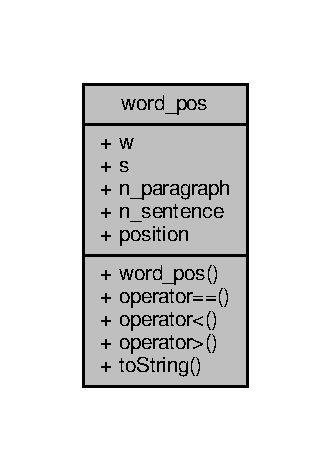
\includegraphics[width=159pt]{structword__pos__coll__graph}
\end{center}
\end{figure}
\subsection*{Public Member Functions}
\begin{DoxyCompactItemize}
\item 
\hyperlink{structword__pos_a1fcd121634f7a9699cc602d73953cef3}{word\+\_\+pos} (const freeling\+::word \&w\+\_\+p, const freeling\+::sentence \&s\+\_\+p, int \hyperlink{structword__pos_a7c6cea15e21d79207980caf3a5b3a81e}{n\+\_\+paragraph}, int \hyperlink{structword__pos_a888700d9397364575480ec17eb0d91c7}{n\+\_\+sentence}, int \hyperlink{structword__pos_a5eaaede340f1d9ca3ac6819b977fd5a1}{position})
\item 
bool \hyperlink{structword__pos_af7b93610dbd7ad40e7e79245acc369b1}{operator==} (\hyperlink{structword__pos}{word\+\_\+pos} other) const 
\begin{DoxyCompactList}\small\item\em Two words are equal if they are in the same position, phrase and paragraph. \end{DoxyCompactList}\item 
bool \hyperlink{structword__pos_a2e03a153eee71b6c9179adf71fcf2f86}{operator$<$} (\hyperlink{structword__pos}{word\+\_\+pos} other) const 
\begin{DoxyCompactList}\small\item\em One word is smaller than other one if it appears later in the text. \end{DoxyCompactList}\item 
bool \hyperlink{structword__pos_abc4a513126b354f38b270026a28c601f}{operator$>$} (\hyperlink{structword__pos}{word\+\_\+pos} other) const 
\begin{DoxyCompactList}\small\item\em One word is greater than other one if it appears sooner in the text. \end{DoxyCompactList}\item 
std\+::wstring \hyperlink{structword__pos_a7027670964b84663d76819a3ff769b44}{to\+String} () const 
\begin{DoxyCompactList}\small\item\em Get a string representation of the \hyperlink{structword__pos}{word\+\_\+pos} to debug. \end{DoxyCompactList}\end{DoxyCompactItemize}
\subsection*{Public Attributes}
\begin{DoxyCompactItemize}
\item 
const freeling\+::word \& \hyperlink{structword__pos_a9268eca742d764f0900d4bfcf7c2720e}{w}
\item 
const freeling\+::sentence \& \hyperlink{structword__pos_a18b13ee20fa43f3e038f76202f5e2f6e}{s}
\item 
int \hyperlink{structword__pos_a7c6cea15e21d79207980caf3a5b3a81e}{n\+\_\+paragraph}
\item 
int \hyperlink{structword__pos_a888700d9397364575480ec17eb0d91c7}{n\+\_\+sentence}
\item 
int \hyperlink{structword__pos_a5eaaede340f1d9ca3ac6819b977fd5a1}{position}
\end{DoxyCompactItemize}


\subsection{Detailed Description}
Struct that allow us to compare words easily. 

\subsection{Constructor \& Destructor Documentation}
\hypertarget{structword__pos_a1fcd121634f7a9699cc602d73953cef3}{}\index{word\+\_\+pos@{word\+\_\+pos}!word\+\_\+pos@{word\+\_\+pos}}
\index{word\+\_\+pos@{word\+\_\+pos}!word\+\_\+pos@{word\+\_\+pos}}
\subsubsection[{word\+\_\+pos}]{\setlength{\rightskip}{0pt plus 5cm}word\+\_\+pos\+::word\+\_\+pos (
\begin{DoxyParamCaption}
\item[{const freeling\+::word \&}]{w\+\_\+p, }
\item[{const freeling\+::sentence \&}]{s\+\_\+p, }
\item[{int}]{n\+\_\+paragraph, }
\item[{int}]{n\+\_\+sentence, }
\item[{int}]{position}
\end{DoxyParamCaption}
)}\label{structword__pos_a1fcd121634f7a9699cc602d73953cef3}


\subsection{Member Function Documentation}
\hypertarget{structword__pos_a2e03a153eee71b6c9179adf71fcf2f86}{}\index{word\+\_\+pos@{word\+\_\+pos}!operator$<$@{operator$<$}}
\index{operator$<$@{operator$<$}!word\+\_\+pos@{word\+\_\+pos}}
\subsubsection[{operator$<$}]{\setlength{\rightskip}{0pt plus 5cm}bool word\+\_\+pos\+::operator$<$ (
\begin{DoxyParamCaption}
\item[{{\bf word\+\_\+pos}}]{other}
\end{DoxyParamCaption}
) const}\label{structword__pos_a2e03a153eee71b6c9179adf71fcf2f86}


One word is smaller than other one if it appears later in the text. 

\hypertarget{structword__pos_af7b93610dbd7ad40e7e79245acc369b1}{}\index{word\+\_\+pos@{word\+\_\+pos}!operator==@{operator==}}
\index{operator==@{operator==}!word\+\_\+pos@{word\+\_\+pos}}
\subsubsection[{operator==}]{\setlength{\rightskip}{0pt plus 5cm}bool word\+\_\+pos\+::operator== (
\begin{DoxyParamCaption}
\item[{{\bf word\+\_\+pos}}]{other}
\end{DoxyParamCaption}
) const}\label{structword__pos_af7b93610dbd7ad40e7e79245acc369b1}


Two words are equal if they are in the same position, phrase and paragraph. 

\hypertarget{structword__pos_abc4a513126b354f38b270026a28c601f}{}\index{word\+\_\+pos@{word\+\_\+pos}!operator$>$@{operator$>$}}
\index{operator$>$@{operator$>$}!word\+\_\+pos@{word\+\_\+pos}}
\subsubsection[{operator$>$}]{\setlength{\rightskip}{0pt plus 5cm}bool word\+\_\+pos\+::operator$>$ (
\begin{DoxyParamCaption}
\item[{{\bf word\+\_\+pos}}]{other}
\end{DoxyParamCaption}
) const}\label{structword__pos_abc4a513126b354f38b270026a28c601f}


One word is greater than other one if it appears sooner in the text. 

\hypertarget{structword__pos_a7027670964b84663d76819a3ff769b44}{}\index{word\+\_\+pos@{word\+\_\+pos}!to\+String@{to\+String}}
\index{to\+String@{to\+String}!word\+\_\+pos@{word\+\_\+pos}}
\subsubsection[{to\+String}]{\setlength{\rightskip}{0pt plus 5cm}wstring word\+\_\+pos\+::to\+String (
\begin{DoxyParamCaption}
{}
\end{DoxyParamCaption}
) const}\label{structword__pos_a7027670964b84663d76819a3ff769b44}


Get a string representation of the \hyperlink{structword__pos}{word\+\_\+pos} to debug. 



\subsection{Member Data Documentation}
\hypertarget{structword__pos_a7c6cea15e21d79207980caf3a5b3a81e}{}\index{word\+\_\+pos@{word\+\_\+pos}!n\+\_\+paragraph@{n\+\_\+paragraph}}
\index{n\+\_\+paragraph@{n\+\_\+paragraph}!word\+\_\+pos@{word\+\_\+pos}}
\subsubsection[{n\+\_\+paragraph}]{\setlength{\rightskip}{0pt plus 5cm}int word\+\_\+pos\+::n\+\_\+paragraph}\label{structword__pos_a7c6cea15e21d79207980caf3a5b3a81e}
\hypertarget{structword__pos_a888700d9397364575480ec17eb0d91c7}{}\index{word\+\_\+pos@{word\+\_\+pos}!n\+\_\+sentence@{n\+\_\+sentence}}
\index{n\+\_\+sentence@{n\+\_\+sentence}!word\+\_\+pos@{word\+\_\+pos}}
\subsubsection[{n\+\_\+sentence}]{\setlength{\rightskip}{0pt plus 5cm}int word\+\_\+pos\+::n\+\_\+sentence}\label{structword__pos_a888700d9397364575480ec17eb0d91c7}
\hypertarget{structword__pos_a5eaaede340f1d9ca3ac6819b977fd5a1}{}\index{word\+\_\+pos@{word\+\_\+pos}!position@{position}}
\index{position@{position}!word\+\_\+pos@{word\+\_\+pos}}
\subsubsection[{position}]{\setlength{\rightskip}{0pt plus 5cm}int word\+\_\+pos\+::position}\label{structword__pos_a5eaaede340f1d9ca3ac6819b977fd5a1}
\hypertarget{structword__pos_a18b13ee20fa43f3e038f76202f5e2f6e}{}\index{word\+\_\+pos@{word\+\_\+pos}!s@{s}}
\index{s@{s}!word\+\_\+pos@{word\+\_\+pos}}
\subsubsection[{s}]{\setlength{\rightskip}{0pt plus 5cm}const freeling\+::sentence\& word\+\_\+pos\+::s}\label{structword__pos_a18b13ee20fa43f3e038f76202f5e2f6e}
\hypertarget{structword__pos_a9268eca742d764f0900d4bfcf7c2720e}{}\index{word\+\_\+pos@{word\+\_\+pos}!w@{w}}
\index{w@{w}!word\+\_\+pos@{word\+\_\+pos}}
\subsubsection[{w}]{\setlength{\rightskip}{0pt plus 5cm}const freeling\+::word\& word\+\_\+pos\+::w}\label{structword__pos_a9268eca742d764f0900d4bfcf7c2720e}


The documentation for this struct was generated from the following files\+:\begin{DoxyCompactItemize}
\item 
\hyperlink{Relation_8h}{Relation.\+h}\item 
\hyperlink{Relation_8cc}{Relation.\+cc}\end{DoxyCompactItemize}

\chapter{File Documentation}
\hypertarget{config_8h}{}\section{/home/samuel/\+Summarizer/src/config.h File Reference}
\label{config_8h}\index{/home/samuel/\+Summarizer/src/config.\+h@{/home/samuel/\+Summarizer/src/config.\+h}}
{\ttfamily \#include $<$exception$>$}\\*
{\ttfamily \#include $<$fstream$>$}\\*
{\ttfamily \#include $<$boost/program\+\_\+options.\+hpp$>$}\\*
{\ttfamily \#include \char`\"{}freeling/version.\+h\char`\"{}}\\*
{\ttfamily \#include \char`\"{}freeling/morfo/traces.\+h\char`\"{}}\\*
{\ttfamily \#include \char`\"{}freeling/morfo/util.\+h\char`\"{}}\\*
{\ttfamily \#include \char`\"{}freeling/morfo/analyzer.\+h\char`\"{}}\\*
Include dependency graph for config.\+h\+:
\nopagebreak
\begin{figure}[H]
\begin{center}
\leavevmode
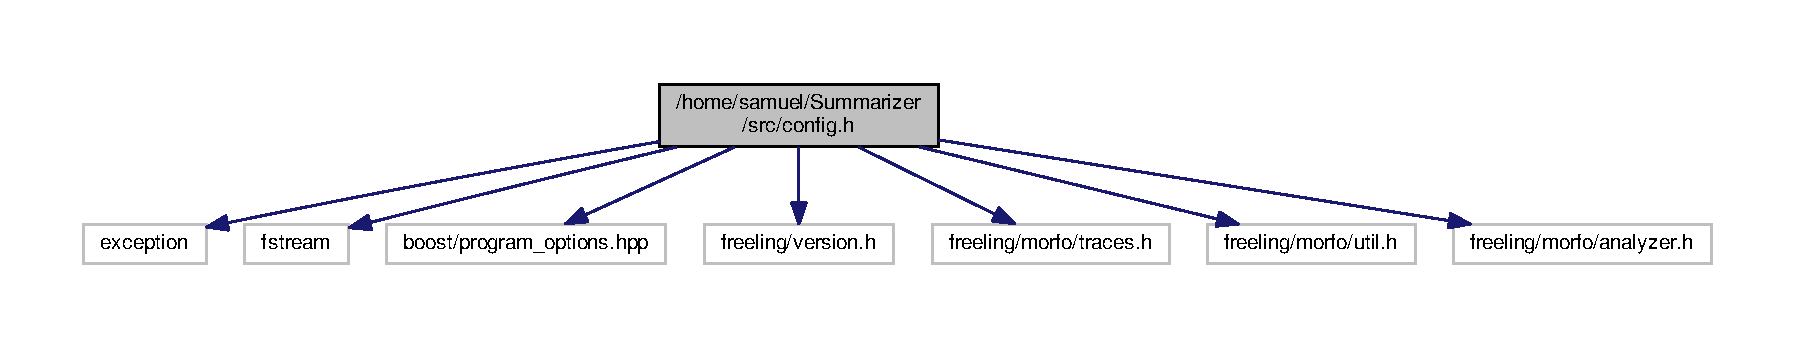
\includegraphics[width=350pt]{config_8h__incl}
\end{center}
\end{figure}
This graph shows which files directly or indirectly include this file\+:
\nopagebreak
\begin{figure}[H]
\begin{center}
\leavevmode
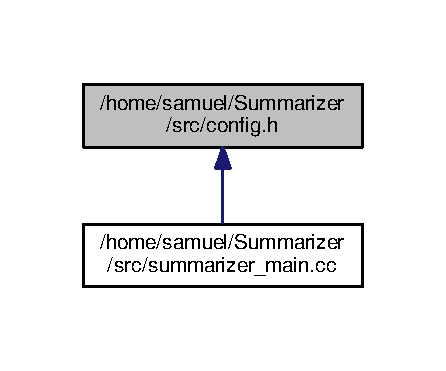
\includegraphics[width=214pt]{config_8h__dep__incl}
\end{center}
\end{figure}
\subsection*{Classes}
\begin{DoxyCompactItemize}
\item 
class \hyperlink{classconfig}{config}
\begin{DoxyCompactList}\small\item\em Class config implements a set of specific options for the N\+L\+P analyzer, providing a C++ wrapper to libcfg+ library. \end{DoxyCompactList}\end{DoxyCompactItemize}
\subsection*{Macros}
\begin{DoxyCompactItemize}
\item 
\#define \hyperlink{config_8h_ab1e34bc45e4737f4c255db28d8616820}{M\+O\+D\+\_\+\+T\+R\+A\+C\+E\+N\+A\+M\+E}~L\char`\"{}C\+O\+N\+F\+I\+G\+\_\+\+O\+P\+T\+I\+O\+N\+S\char`\"{}
\item 
\#define \hyperlink{config_8h_a6dc0328a20069cd8c23a96d082081a9d}{D\+E\+F\+A\+U\+L\+T\+\_\+\+M\+A\+X\+\_\+\+W\+O\+R\+K\+E\+R\+S}~5
\item 
\#define \hyperlink{config_8h_a9bb74553a93bc7f4c7c94a6b0e1d07dc}{D\+E\+F\+A\+U\+L\+T\+\_\+\+Q\+U\+E\+U\+E\+\_\+\+S\+I\+Z\+E}~32
\end{DoxyCompactItemize}
\subsection*{Enumerations}
\begin{DoxyCompactItemize}
\item 
enum \hyperlink{config_8h_ad5cac7b85d200232841f3f0a31bea5c1}{Input\+Modes} \{ \hyperlink{config_8h_ad5cac7b85d200232841f3f0a31bea5c1afb101bbdd2ec7527a67723a0393c1f8f}{M\+O\+D\+E\+\_\+\+C\+O\+R\+P\+U\+S}, 
\hyperlink{config_8h_ad5cac7b85d200232841f3f0a31bea5c1a39e54696ba50be485ee400e051f9e37d}{M\+O\+D\+E\+\_\+\+D\+O\+C}
 \}
\item 
enum \hyperlink{config_8h_a3f8677a5e7c7cdae9eae3f84e38bd5bd}{Output\+Formats} \{ \\*
\hyperlink{config_8h_a3f8677a5e7c7cdae9eae3f84e38bd5bda391e4d2b4cb2bf288b76acde9b034d2f}{O\+U\+T\+\_\+\+F\+R\+E\+E\+L\+I\+N\+G}, 
\hyperlink{config_8h_a3f8677a5e7c7cdae9eae3f84e38bd5bdaf9d732862e4474bee4597bd7e91e64c3}{O\+U\+T\+\_\+\+T\+R\+A\+I\+N}, 
\hyperlink{config_8h_a3f8677a5e7c7cdae9eae3f84e38bd5bda8e7f2f84b4bb6b79a93c823585054568}{O\+U\+T\+\_\+\+C\+O\+N\+L\+L}, 
\hyperlink{config_8h_a3f8677a5e7c7cdae9eae3f84e38bd5bdaa4864f7504e83bf99d0f2377fce82bf5}{O\+U\+T\+\_\+\+X\+M\+L}, 
\\*
\hyperlink{config_8h_a3f8677a5e7c7cdae9eae3f84e38bd5bda25cff6f8efbef938ac952d30957e7329}{O\+U\+T\+\_\+\+J\+S\+O\+N}, 
\hyperlink{config_8h_a3f8677a5e7c7cdae9eae3f84e38bd5bda25f6a19fc545a3a34fe80207a487b127}{O\+U\+T\+\_\+\+N\+A\+F}
 \}
\item 
enum \hyperlink{config_8h_aa29a34e3d6e44b1b5d909fb8cfcfdfb6}{Input\+Formats} \{ \hyperlink{config_8h_aa29a34e3d6e44b1b5d909fb8cfcfdfb6abc10178a6b5b03f555bc15327469a929}{I\+N\+P\+\_\+\+T\+E\+X\+T}, 
\hyperlink{config_8h_aa29a34e3d6e44b1b5d909fb8cfcfdfb6a2e8a8d0ba33af3cd96cf2c9db651115e}{I\+N\+P\+\_\+\+F\+R\+E\+E\+L\+I\+N\+G}, 
\hyperlink{config_8h_aa29a34e3d6e44b1b5d909fb8cfcfdfb6a6ab747ee5d9646a8e4662828cce53d39}{I\+N\+P\+\_\+\+C\+O\+N\+L\+L}
 \}
\end{DoxyCompactItemize}


\subsection{Macro Definition Documentation}
\hypertarget{config_8h_a6dc0328a20069cd8c23a96d082081a9d}{}\index{config.\+h@{config.\+h}!D\+E\+F\+A\+U\+L\+T\+\_\+\+M\+A\+X\+\_\+\+W\+O\+R\+K\+E\+R\+S@{D\+E\+F\+A\+U\+L\+T\+\_\+\+M\+A\+X\+\_\+\+W\+O\+R\+K\+E\+R\+S}}
\index{D\+E\+F\+A\+U\+L\+T\+\_\+\+M\+A\+X\+\_\+\+W\+O\+R\+K\+E\+R\+S@{D\+E\+F\+A\+U\+L\+T\+\_\+\+M\+A\+X\+\_\+\+W\+O\+R\+K\+E\+R\+S}!config.\+h@{config.\+h}}
\subsubsection[{D\+E\+F\+A\+U\+L\+T\+\_\+\+M\+A\+X\+\_\+\+W\+O\+R\+K\+E\+R\+S}]{\setlength{\rightskip}{0pt plus 5cm}\#define D\+E\+F\+A\+U\+L\+T\+\_\+\+M\+A\+X\+\_\+\+W\+O\+R\+K\+E\+R\+S~5}\label{config_8h_a6dc0328a20069cd8c23a96d082081a9d}
\hypertarget{config_8h_a9bb74553a93bc7f4c7c94a6b0e1d07dc}{}\index{config.\+h@{config.\+h}!D\+E\+F\+A\+U\+L\+T\+\_\+\+Q\+U\+E\+U\+E\+\_\+\+S\+I\+Z\+E@{D\+E\+F\+A\+U\+L\+T\+\_\+\+Q\+U\+E\+U\+E\+\_\+\+S\+I\+Z\+E}}
\index{D\+E\+F\+A\+U\+L\+T\+\_\+\+Q\+U\+E\+U\+E\+\_\+\+S\+I\+Z\+E@{D\+E\+F\+A\+U\+L\+T\+\_\+\+Q\+U\+E\+U\+E\+\_\+\+S\+I\+Z\+E}!config.\+h@{config.\+h}}
\subsubsection[{D\+E\+F\+A\+U\+L\+T\+\_\+\+Q\+U\+E\+U\+E\+\_\+\+S\+I\+Z\+E}]{\setlength{\rightskip}{0pt plus 5cm}\#define D\+E\+F\+A\+U\+L\+T\+\_\+\+Q\+U\+E\+U\+E\+\_\+\+S\+I\+Z\+E~32}\label{config_8h_a9bb74553a93bc7f4c7c94a6b0e1d07dc}
\hypertarget{config_8h_ab1e34bc45e4737f4c255db28d8616820}{}\index{config.\+h@{config.\+h}!M\+O\+D\+\_\+\+T\+R\+A\+C\+E\+N\+A\+M\+E@{M\+O\+D\+\_\+\+T\+R\+A\+C\+E\+N\+A\+M\+E}}
\index{M\+O\+D\+\_\+\+T\+R\+A\+C\+E\+N\+A\+M\+E@{M\+O\+D\+\_\+\+T\+R\+A\+C\+E\+N\+A\+M\+E}!config.\+h@{config.\+h}}
\subsubsection[{M\+O\+D\+\_\+\+T\+R\+A\+C\+E\+N\+A\+M\+E}]{\setlength{\rightskip}{0pt plus 5cm}\#define M\+O\+D\+\_\+\+T\+R\+A\+C\+E\+N\+A\+M\+E~L\char`\"{}C\+O\+N\+F\+I\+G\+\_\+\+O\+P\+T\+I\+O\+N\+S\char`\"{}}\label{config_8h_ab1e34bc45e4737f4c255db28d8616820}


\subsection{Enumeration Type Documentation}
\hypertarget{config_8h_aa29a34e3d6e44b1b5d909fb8cfcfdfb6}{}\index{config.\+h@{config.\+h}!Input\+Formats@{Input\+Formats}}
\index{Input\+Formats@{Input\+Formats}!config.\+h@{config.\+h}}
\subsubsection[{Input\+Formats}]{\setlength{\rightskip}{0pt plus 5cm}enum {\bf Input\+Formats}}\label{config_8h_aa29a34e3d6e44b1b5d909fb8cfcfdfb6}
\begin{Desc}
\item[Enumerator]\par
\begin{description}
\index{I\+N\+P\+\_\+\+T\+E\+X\+T@{I\+N\+P\+\_\+\+T\+E\+X\+T}!config.\+h@{config.\+h}}\index{config.\+h@{config.\+h}!I\+N\+P\+\_\+\+T\+E\+X\+T@{I\+N\+P\+\_\+\+T\+E\+X\+T}}\item[{\em 
\hypertarget{config_8h_aa29a34e3d6e44b1b5d909fb8cfcfdfb6abc10178a6b5b03f555bc15327469a929}{}I\+N\+P\+\_\+\+T\+E\+X\+T\label{config_8h_aa29a34e3d6e44b1b5d909fb8cfcfdfb6abc10178a6b5b03f555bc15327469a929}
}]\index{I\+N\+P\+\_\+\+F\+R\+E\+E\+L\+I\+N\+G@{I\+N\+P\+\_\+\+F\+R\+E\+E\+L\+I\+N\+G}!config.\+h@{config.\+h}}\index{config.\+h@{config.\+h}!I\+N\+P\+\_\+\+F\+R\+E\+E\+L\+I\+N\+G@{I\+N\+P\+\_\+\+F\+R\+E\+E\+L\+I\+N\+G}}\item[{\em 
\hypertarget{config_8h_aa29a34e3d6e44b1b5d909fb8cfcfdfb6a2e8a8d0ba33af3cd96cf2c9db651115e}{}I\+N\+P\+\_\+\+F\+R\+E\+E\+L\+I\+N\+G\label{config_8h_aa29a34e3d6e44b1b5d909fb8cfcfdfb6a2e8a8d0ba33af3cd96cf2c9db651115e}
}]\index{I\+N\+P\+\_\+\+C\+O\+N\+L\+L@{I\+N\+P\+\_\+\+C\+O\+N\+L\+L}!config.\+h@{config.\+h}}\index{config.\+h@{config.\+h}!I\+N\+P\+\_\+\+C\+O\+N\+L\+L@{I\+N\+P\+\_\+\+C\+O\+N\+L\+L}}\item[{\em 
\hypertarget{config_8h_aa29a34e3d6e44b1b5d909fb8cfcfdfb6a6ab747ee5d9646a8e4662828cce53d39}{}I\+N\+P\+\_\+\+C\+O\+N\+L\+L\label{config_8h_aa29a34e3d6e44b1b5d909fb8cfcfdfb6a6ab747ee5d9646a8e4662828cce53d39}
}]\end{description}
\end{Desc}
\hypertarget{config_8h_ad5cac7b85d200232841f3f0a31bea5c1}{}\index{config.\+h@{config.\+h}!Input\+Modes@{Input\+Modes}}
\index{Input\+Modes@{Input\+Modes}!config.\+h@{config.\+h}}
\subsubsection[{Input\+Modes}]{\setlength{\rightskip}{0pt plus 5cm}enum {\bf Input\+Modes}}\label{config_8h_ad5cac7b85d200232841f3f0a31bea5c1}
\begin{Desc}
\item[Enumerator]\par
\begin{description}
\index{M\+O\+D\+E\+\_\+\+C\+O\+R\+P\+U\+S@{M\+O\+D\+E\+\_\+\+C\+O\+R\+P\+U\+S}!config.\+h@{config.\+h}}\index{config.\+h@{config.\+h}!M\+O\+D\+E\+\_\+\+C\+O\+R\+P\+U\+S@{M\+O\+D\+E\+\_\+\+C\+O\+R\+P\+U\+S}}\item[{\em 
\hypertarget{config_8h_ad5cac7b85d200232841f3f0a31bea5c1afb101bbdd2ec7527a67723a0393c1f8f}{}M\+O\+D\+E\+\_\+\+C\+O\+R\+P\+U\+S\label{config_8h_ad5cac7b85d200232841f3f0a31bea5c1afb101bbdd2ec7527a67723a0393c1f8f}
}]\index{M\+O\+D\+E\+\_\+\+D\+O\+C@{M\+O\+D\+E\+\_\+\+D\+O\+C}!config.\+h@{config.\+h}}\index{config.\+h@{config.\+h}!M\+O\+D\+E\+\_\+\+D\+O\+C@{M\+O\+D\+E\+\_\+\+D\+O\+C}}\item[{\em 
\hypertarget{config_8h_ad5cac7b85d200232841f3f0a31bea5c1a39e54696ba50be485ee400e051f9e37d}{}M\+O\+D\+E\+\_\+\+D\+O\+C\label{config_8h_ad5cac7b85d200232841f3f0a31bea5c1a39e54696ba50be485ee400e051f9e37d}
}]\end{description}
\end{Desc}
\hypertarget{config_8h_a3f8677a5e7c7cdae9eae3f84e38bd5bd}{}\index{config.\+h@{config.\+h}!Output\+Formats@{Output\+Formats}}
\index{Output\+Formats@{Output\+Formats}!config.\+h@{config.\+h}}
\subsubsection[{Output\+Formats}]{\setlength{\rightskip}{0pt plus 5cm}enum {\bf Output\+Formats}}\label{config_8h_a3f8677a5e7c7cdae9eae3f84e38bd5bd}
\begin{Desc}
\item[Enumerator]\par
\begin{description}
\index{O\+U\+T\+\_\+\+F\+R\+E\+E\+L\+I\+N\+G@{O\+U\+T\+\_\+\+F\+R\+E\+E\+L\+I\+N\+G}!config.\+h@{config.\+h}}\index{config.\+h@{config.\+h}!O\+U\+T\+\_\+\+F\+R\+E\+E\+L\+I\+N\+G@{O\+U\+T\+\_\+\+F\+R\+E\+E\+L\+I\+N\+G}}\item[{\em 
\hypertarget{config_8h_a3f8677a5e7c7cdae9eae3f84e38bd5bda391e4d2b4cb2bf288b76acde9b034d2f}{}O\+U\+T\+\_\+\+F\+R\+E\+E\+L\+I\+N\+G\label{config_8h_a3f8677a5e7c7cdae9eae3f84e38bd5bda391e4d2b4cb2bf288b76acde9b034d2f}
}]\index{O\+U\+T\+\_\+\+T\+R\+A\+I\+N@{O\+U\+T\+\_\+\+T\+R\+A\+I\+N}!config.\+h@{config.\+h}}\index{config.\+h@{config.\+h}!O\+U\+T\+\_\+\+T\+R\+A\+I\+N@{O\+U\+T\+\_\+\+T\+R\+A\+I\+N}}\item[{\em 
\hypertarget{config_8h_a3f8677a5e7c7cdae9eae3f84e38bd5bdaf9d732862e4474bee4597bd7e91e64c3}{}O\+U\+T\+\_\+\+T\+R\+A\+I\+N\label{config_8h_a3f8677a5e7c7cdae9eae3f84e38bd5bdaf9d732862e4474bee4597bd7e91e64c3}
}]\index{O\+U\+T\+\_\+\+C\+O\+N\+L\+L@{O\+U\+T\+\_\+\+C\+O\+N\+L\+L}!config.\+h@{config.\+h}}\index{config.\+h@{config.\+h}!O\+U\+T\+\_\+\+C\+O\+N\+L\+L@{O\+U\+T\+\_\+\+C\+O\+N\+L\+L}}\item[{\em 
\hypertarget{config_8h_a3f8677a5e7c7cdae9eae3f84e38bd5bda8e7f2f84b4bb6b79a93c823585054568}{}O\+U\+T\+\_\+\+C\+O\+N\+L\+L\label{config_8h_a3f8677a5e7c7cdae9eae3f84e38bd5bda8e7f2f84b4bb6b79a93c823585054568}
}]\index{O\+U\+T\+\_\+\+X\+M\+L@{O\+U\+T\+\_\+\+X\+M\+L}!config.\+h@{config.\+h}}\index{config.\+h@{config.\+h}!O\+U\+T\+\_\+\+X\+M\+L@{O\+U\+T\+\_\+\+X\+M\+L}}\item[{\em 
\hypertarget{config_8h_a3f8677a5e7c7cdae9eae3f84e38bd5bdaa4864f7504e83bf99d0f2377fce82bf5}{}O\+U\+T\+\_\+\+X\+M\+L\label{config_8h_a3f8677a5e7c7cdae9eae3f84e38bd5bdaa4864f7504e83bf99d0f2377fce82bf5}
}]\index{O\+U\+T\+\_\+\+J\+S\+O\+N@{O\+U\+T\+\_\+\+J\+S\+O\+N}!config.\+h@{config.\+h}}\index{config.\+h@{config.\+h}!O\+U\+T\+\_\+\+J\+S\+O\+N@{O\+U\+T\+\_\+\+J\+S\+O\+N}}\item[{\em 
\hypertarget{config_8h_a3f8677a5e7c7cdae9eae3f84e38bd5bda25cff6f8efbef938ac952d30957e7329}{}O\+U\+T\+\_\+\+J\+S\+O\+N\label{config_8h_a3f8677a5e7c7cdae9eae3f84e38bd5bda25cff6f8efbef938ac952d30957e7329}
}]\index{O\+U\+T\+\_\+\+N\+A\+F@{O\+U\+T\+\_\+\+N\+A\+F}!config.\+h@{config.\+h}}\index{config.\+h@{config.\+h}!O\+U\+T\+\_\+\+N\+A\+F@{O\+U\+T\+\_\+\+N\+A\+F}}\item[{\em 
\hypertarget{config_8h_a3f8677a5e7c7cdae9eae3f84e38bd5bda25f6a19fc545a3a34fe80207a487b127}{}O\+U\+T\+\_\+\+N\+A\+F\label{config_8h_a3f8677a5e7c7cdae9eae3f84e38bd5bda25f6a19fc545a3a34fe80207a487b127}
}]\end{description}
\end{Desc}

\hypertarget{LexicalChain_8cc}{}\section{Lexical\+Chain.\+cc File Reference}
\label{LexicalChain_8cc}\index{Lexical\+Chain.\+cc@{Lexical\+Chain.\+cc}}
{\ttfamily \#include \char`\"{}Lexical\+Chain.\+h\char`\"{}}\\*
Include dependency graph for Lexical\+Chain.\+cc\+:\nopagebreak
\begin{figure}[H]
\begin{center}
\leavevmode
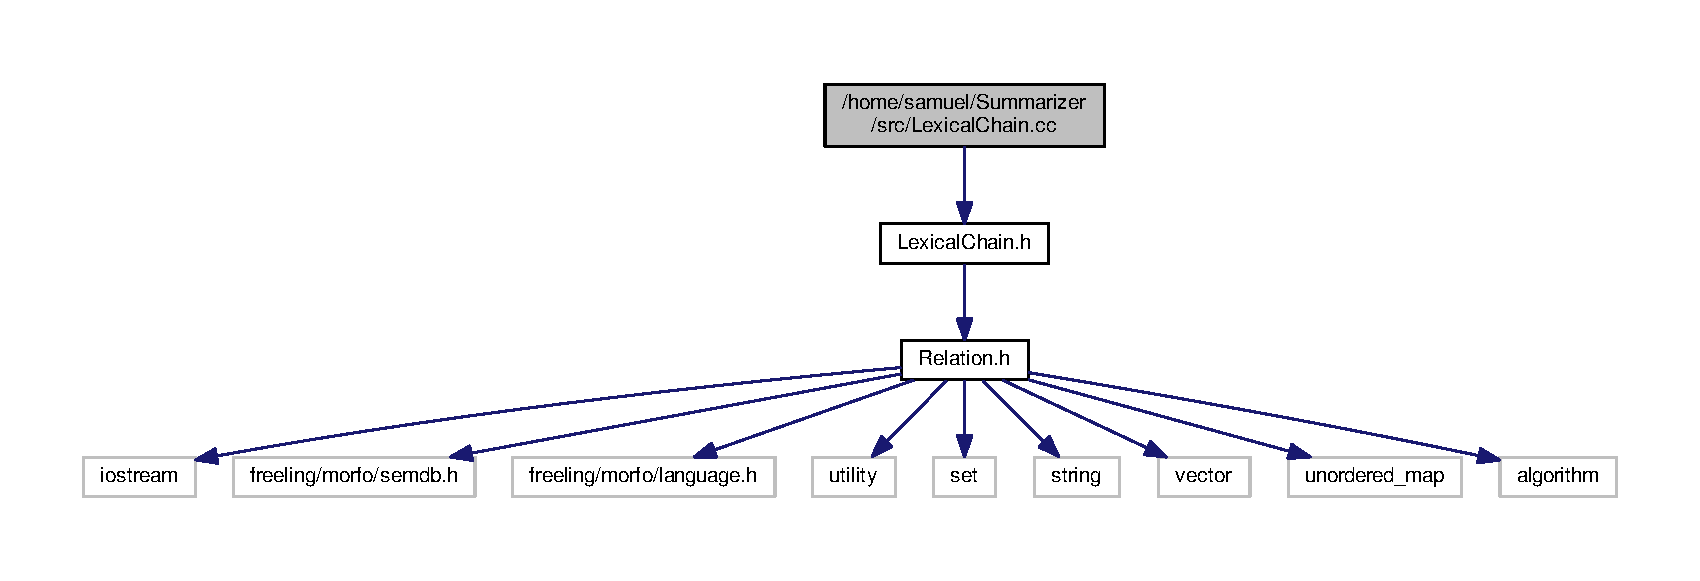
\includegraphics[width=350pt]{LexicalChain_8cc__incl}
\end{center}
\end{figure}

\hypertarget{LexicalChain_8h}{}\section{Lexical\+Chain.\+h File Reference}
\label{LexicalChain_8h}\index{Lexical\+Chain.\+h@{Lexical\+Chain.\+h}}
{\ttfamily \#include \char`\"{}Relation.\+h\char`\"{}}\\*
Include dependency graph for Lexical\+Chain.\+h\+:\nopagebreak
\begin{figure}[H]
\begin{center}
\leavevmode
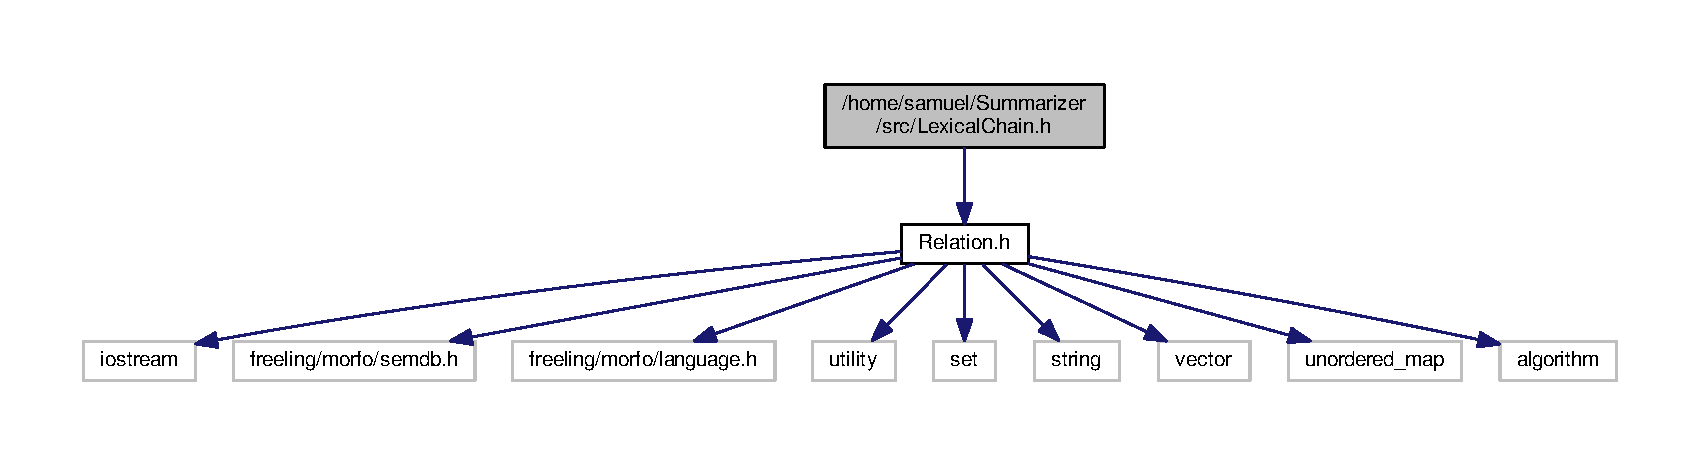
\includegraphics[width=350pt]{LexicalChain_8h__incl}
\end{center}
\end{figure}
This graph shows which files directly or indirectly include this file\+:\nopagebreak
\begin{figure}[H]
\begin{center}
\leavevmode
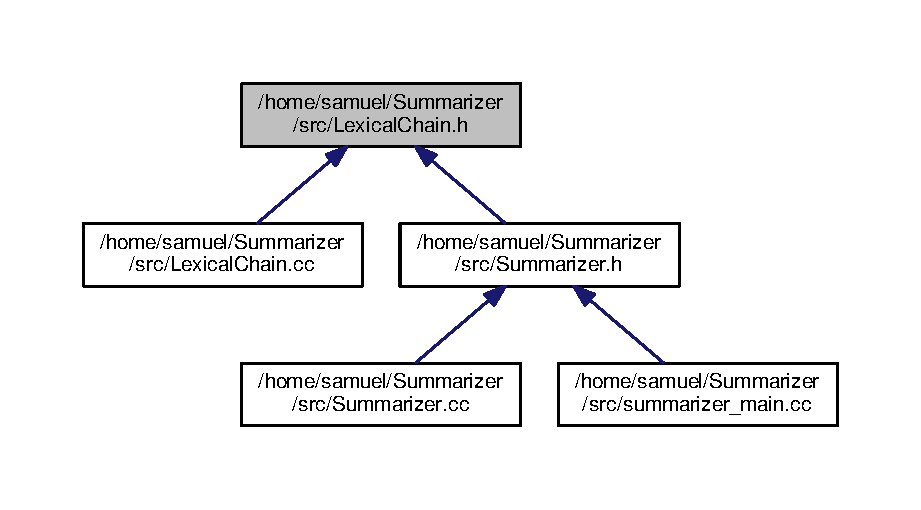
\includegraphics[width=334pt]{LexicalChain_8h__dep__incl}
\end{center}
\end{figure}
\subsection*{Classes}
\begin{DoxyCompactItemize}
\item 
class \hyperlink{classLexicalChain}{Lexical\+Chain}
\begin{DoxyCompactList}\small\item\em Class \hyperlink{classLexicalChain}{Lexical\+Chain} represents a lexical chain and computes words and stores (or not) them into the structures. \end{DoxyCompactList}\end{DoxyCompactItemize}

\hypertarget{Relation_8cc}{}\section{/home/samuel/\+Summarizer/src/\+Relation.cc File Reference}
\label{Relation_8cc}\index{/home/samuel/\+Summarizer/src/\+Relation.\+cc@{/home/samuel/\+Summarizer/src/\+Relation.\+cc}}
{\ttfamily \#include \char`\"{}Relation.\+h\char`\"{}}\\*
Include dependency graph for Relation.\+cc\+:
\nopagebreak
\begin{figure}[H]
\begin{center}
\leavevmode
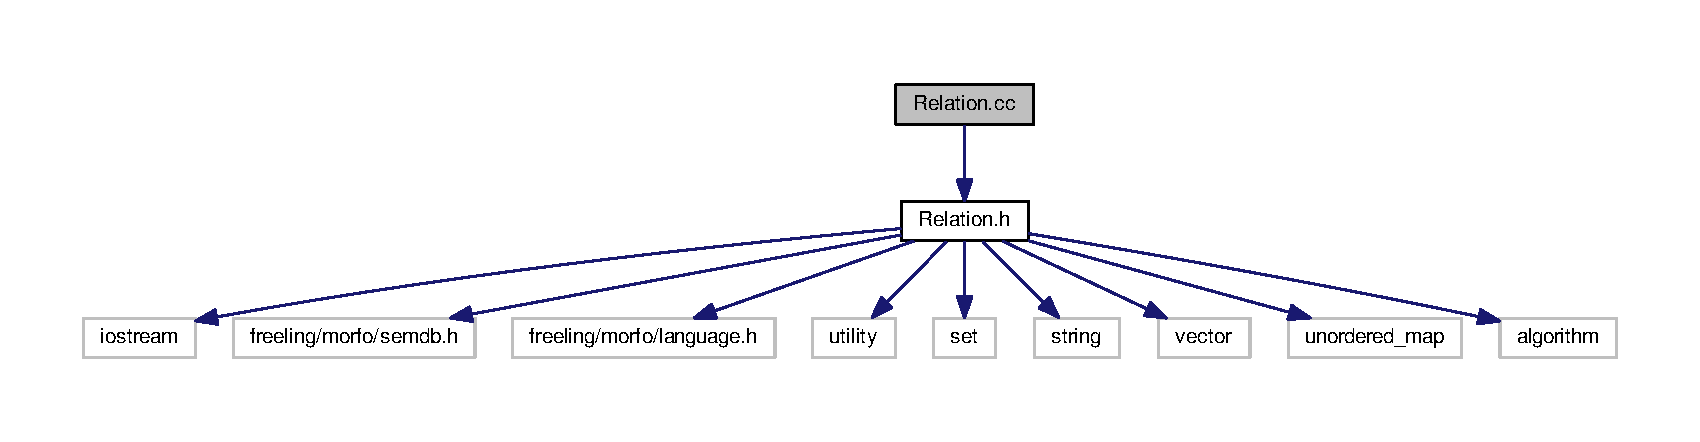
\includegraphics[width=350pt]{Relation_8cc__incl}
\end{center}
\end{figure}
\subsection*{Functions}
\begin{DoxyCompactItemize}
\item 
bool \hyperlink{Relation_8cc_aa4dedffae1bb00e5555d2b8643405530}{order\+\_\+by\+\_\+score} (const pair$<$ int, \hyperlink{structword__pos}{word\+\_\+pos} $\ast$ $>$ \&p1, const pair$<$ int, \hyperlink{structword__pos}{word\+\_\+pos} $\ast$ $>$ \&p2)
\item 
bool \hyperlink{Relation_8cc_a7fcaee1d794ef02cf968e454b0698f5c}{order\+\_\+by\+\_\+tag\+\_\+and\+\_\+score} (const pair$<$ int, \hyperlink{structword__pos}{word\+\_\+pos} $\ast$ $>$ \&p1, const pair$<$ int, \hyperlink{structword__pos}{word\+\_\+pos} $\ast$ $>$ \&p2)
\end{DoxyCompactItemize}


\subsection{Function Documentation}
\hypertarget{Relation_8cc_aa4dedffae1bb00e5555d2b8643405530}{}\index{Relation.\+cc@{Relation.\+cc}!order\+\_\+by\+\_\+score@{order\+\_\+by\+\_\+score}}
\index{order\+\_\+by\+\_\+score@{order\+\_\+by\+\_\+score}!Relation.\+cc@{Relation.\+cc}}
\subsubsection[{order\+\_\+by\+\_\+score}]{\setlength{\rightskip}{0pt plus 5cm}bool order\+\_\+by\+\_\+score (
\begin{DoxyParamCaption}
\item[{const pair$<$ int, {\bf word\+\_\+pos} $\ast$ $>$ \&}]{p1, }
\item[{const pair$<$ int, {\bf word\+\_\+pos} $\ast$ $>$ \&}]{p2}
\end{DoxyParamCaption}
)}\label{Relation_8cc_aa4dedffae1bb00e5555d2b8643405530}
\hypertarget{Relation_8cc_a7fcaee1d794ef02cf968e454b0698f5c}{}\index{Relation.\+cc@{Relation.\+cc}!order\+\_\+by\+\_\+tag\+\_\+and\+\_\+score@{order\+\_\+by\+\_\+tag\+\_\+and\+\_\+score}}
\index{order\+\_\+by\+\_\+tag\+\_\+and\+\_\+score@{order\+\_\+by\+\_\+tag\+\_\+and\+\_\+score}!Relation.\+cc@{Relation.\+cc}}
\subsubsection[{order\+\_\+by\+\_\+tag\+\_\+and\+\_\+score}]{\setlength{\rightskip}{0pt plus 5cm}bool order\+\_\+by\+\_\+tag\+\_\+and\+\_\+score (
\begin{DoxyParamCaption}
\item[{const pair$<$ int, {\bf word\+\_\+pos} $\ast$ $>$ \&}]{p1, }
\item[{const pair$<$ int, {\bf word\+\_\+pos} $\ast$ $>$ \&}]{p2}
\end{DoxyParamCaption}
)}\label{Relation_8cc_a7fcaee1d794ef02cf968e454b0698f5c}

\hypertarget{Relation_8h}{}\section{/home/samuel/\+Summarizer/src/\+Relation.h File Reference}
\label{Relation_8h}\index{/home/samuel/\+Summarizer/src/\+Relation.\+h@{/home/samuel/\+Summarizer/src/\+Relation.\+h}}
{\ttfamily \#include $<$iostream$>$}\\*
{\ttfamily \#include \char`\"{}freeling/morfo/semdb.\+h\char`\"{}}\\*
{\ttfamily \#include \char`\"{}freeling/morfo/language.\+h\char`\"{}}\\*
{\ttfamily \#include $<$utility$>$}\\*
{\ttfamily \#include $<$set$>$}\\*
{\ttfamily \#include $<$string$>$}\\*
{\ttfamily \#include $<$vector$>$}\\*
{\ttfamily \#include $<$unordered\+\_\+map$>$}\\*
{\ttfamily \#include $<$algorithm$>$}\\*
Include dependency graph for Relation.\+h\+:
\nopagebreak
\begin{figure}[H]
\begin{center}
\leavevmode
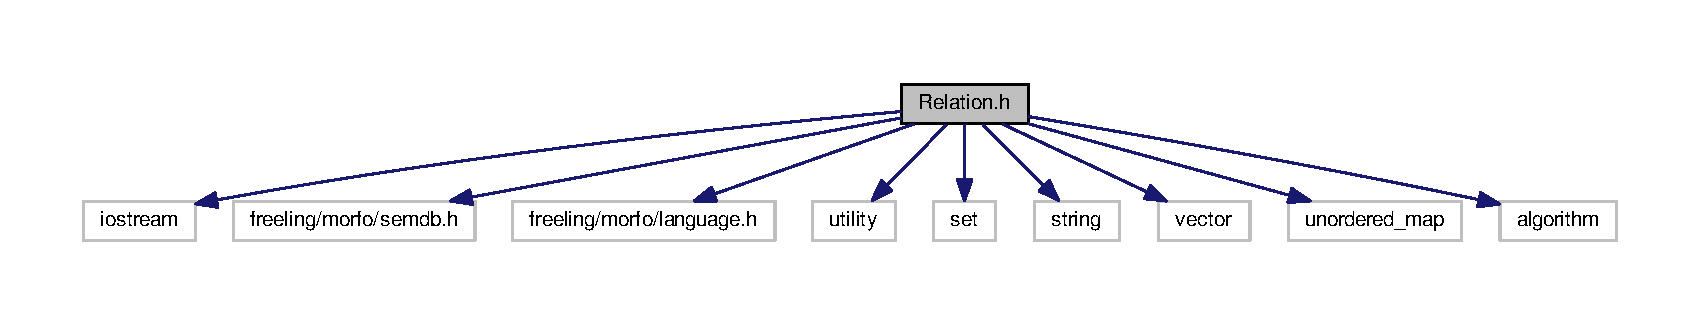
\includegraphics[width=350pt]{Relation_8h__incl}
\end{center}
\end{figure}
This graph shows which files directly or indirectly include this file\+:
\nopagebreak
\begin{figure}[H]
\begin{center}
\leavevmode
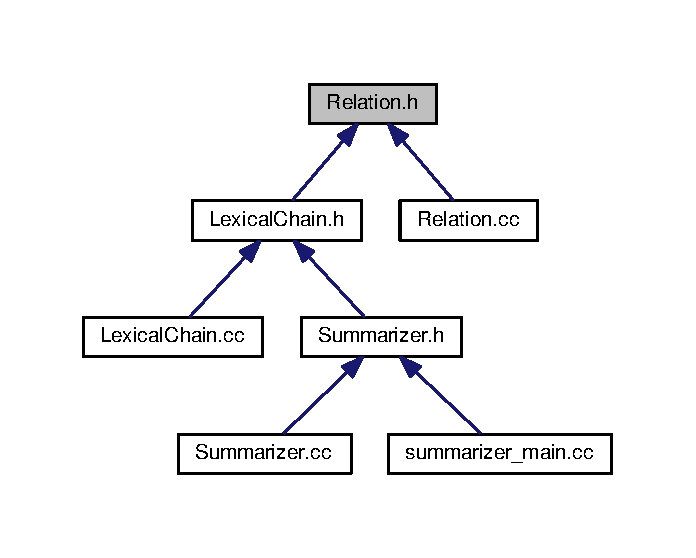
\includegraphics[width=350pt]{Relation_8h__dep__incl}
\end{center}
\end{figure}
\subsection*{Classes}
\begin{DoxyCompactItemize}
\item 
struct \hyperlink{structword__pos}{word\+\_\+pos}
\begin{DoxyCompactList}\small\item\em Struct that allow us to compare words easily. \end{DoxyCompactList}\item 
struct \hyperlink{structrelated__words}{related\+\_\+words}
\begin{DoxyCompactList}\small\item\em Struct that represents a relationship between two words. \end{DoxyCompactList}\item 
class \hyperlink{classRelation}{Relation}
\begin{DoxyCompactList}\small\item\em Class \hyperlink{classRelation}{Relation} is a non-\/instantiable class which defines many virtual methods to check if a word is compatible with the \hyperlink{classRelation}{Relation} or if a word can be stored in the structures of a lexical chain. \end{DoxyCompactList}\item 
class \hyperlink{classSameWord}{Same\+Word}
\begin{DoxyCompactList}\small\item\em Class \hyperlink{classSameWord}{Same\+Word} represents the same word relation\+: two words are related if they are the same word. \end{DoxyCompactList}\item 
class \hyperlink{classHypernymy}{Hypernymy}
\begin{DoxyCompactList}\small\item\em Class \hyperlink{classHypernymy}{Hypernymy} represents the hypernymy relation\+: two words are related if one is an hypernymy of the other and the hypernymy depth is smaller or equal than a given maximum. \end{DoxyCompactList}\item 
class \hyperlink{classSameCorefGroup}{Same\+Coref\+Group}
\begin{DoxyCompactList}\small\item\em Class \hyperlink{classSameCorefGroup}{Same\+Coref\+Group} represents the same coreference group relation\+: two words are related if they are in the same coreference group. \end{DoxyCompactList}\end{DoxyCompactItemize}

\hypertarget{Summarizer_8cc}{}\section{Summarizer.\+cc File Reference}
\label{Summarizer_8cc}\index{Summarizer.\+cc@{Summarizer.\+cc}}
{\ttfamily \#include \char`\"{}Summarizer.\+h\char`\"{}}\\*
Include dependency graph for Summarizer.\+cc\+:\nopagebreak
\begin{figure}[H]
\begin{center}
\leavevmode
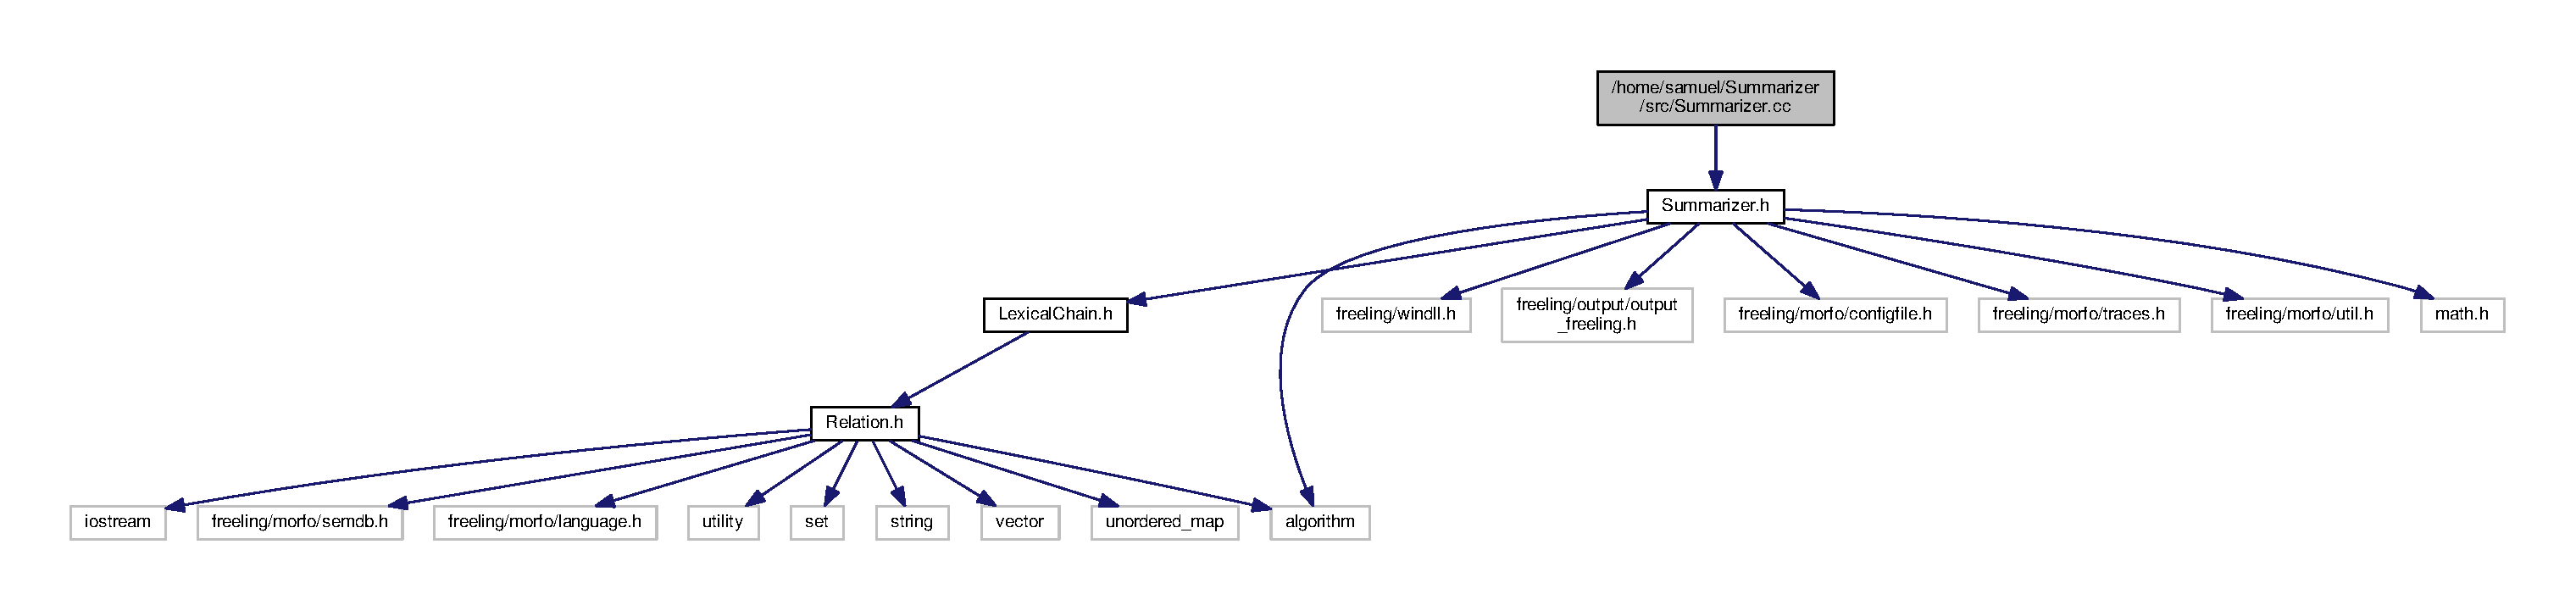
\includegraphics[width=350pt]{Summarizer_8cc__incl}
\end{center}
\end{figure}
\subsection*{Functions}
\begin{DoxyCompactItemize}
\item 
bool \hyperlink{Summarizer_8cc_ae4278069beebfacf507b6c5be86bad41}{compare\+\_\+lexical\+\_\+chains} (\hyperlink{classLexicalChain}{Lexical\+Chain} \&first, \hyperlink{classLexicalChain}{Lexical\+Chain} \&second)
\item 
bool \hyperlink{Summarizer_8cc_abbfb2eb07ca8e54c527b9d82ce054c17}{order\+\_\+by\+\_\+scores} (const pair$<$ int, const \hyperlink{structword__pos}{word\+\_\+pos} $\ast$ $>$ \&sc\+\_\+wp1, const pair$<$ int, const \hyperlink{structword__pos}{word\+\_\+pos} $\ast$ $>$ \&sc\+\_\+wp2)
\end{DoxyCompactItemize}


\subsection{Function Documentation}
\hypertarget{Summarizer_8cc_ae4278069beebfacf507b6c5be86bad41}{}\index{Summarizer.\+cc@{Summarizer.\+cc}!compare\+\_\+lexical\+\_\+chains@{compare\+\_\+lexical\+\_\+chains}}
\index{compare\+\_\+lexical\+\_\+chains@{compare\+\_\+lexical\+\_\+chains}!Summarizer.\+cc@{Summarizer.\+cc}}
\subsubsection[{compare\+\_\+lexical\+\_\+chains}]{\setlength{\rightskip}{0pt plus 5cm}bool compare\+\_\+lexical\+\_\+chains (
\begin{DoxyParamCaption}
\item[{{\bf Lexical\+Chain} \&}]{first, }
\item[{{\bf Lexical\+Chain} \&}]{second}
\end{DoxyParamCaption}
)}\label{Summarizer_8cc_ae4278069beebfacf507b6c5be86bad41}
\hypertarget{Summarizer_8cc_abbfb2eb07ca8e54c527b9d82ce054c17}{}\index{Summarizer.\+cc@{Summarizer.\+cc}!order\+\_\+by\+\_\+scores@{order\+\_\+by\+\_\+scores}}
\index{order\+\_\+by\+\_\+scores@{order\+\_\+by\+\_\+scores}!Summarizer.\+cc@{Summarizer.\+cc}}
\subsubsection[{order\+\_\+by\+\_\+scores}]{\setlength{\rightskip}{0pt plus 5cm}bool order\+\_\+by\+\_\+scores (
\begin{DoxyParamCaption}
\item[{const pair$<$ int, const {\bf word\+\_\+pos} $\ast$ $>$ \&}]{sc\+\_\+wp1, }
\item[{const pair$<$ int, const {\bf word\+\_\+pos} $\ast$ $>$ \&}]{sc\+\_\+wp2}
\end{DoxyParamCaption}
)}\label{Summarizer_8cc_abbfb2eb07ca8e54c527b9d82ce054c17}

\hypertarget{Summarizer_8h}{}\section{Summarizer.\+h File Reference}
\label{Summarizer_8h}\index{Summarizer.\+h@{Summarizer.\+h}}
{\ttfamily \#include \char`\"{}Lexical\+Chain.\+h\char`\"{}}\\*
{\ttfamily \#include \char`\"{}freeling/windll.\+h\char`\"{}}\\*
{\ttfamily \#include \char`\"{}freeling/output/output\+\_\+freeling.\+h\char`\"{}}\\*
{\ttfamily \#include \char`\"{}freeling/morfo/configfile.\+h\char`\"{}}\\*
{\ttfamily \#include \char`\"{}freeling/morfo/traces.\+h\char`\"{}}\\*
{\ttfamily \#include \char`\"{}freeling/morfo/util.\+h\char`\"{}}\\*
{\ttfamily \#include $<$algorithm$>$}\\*
{\ttfamily \#include $<$math.\+h$>$}\\*
Include dependency graph for Summarizer.\+h\+:
\nopagebreak
\begin{figure}[H]
\begin{center}
\leavevmode
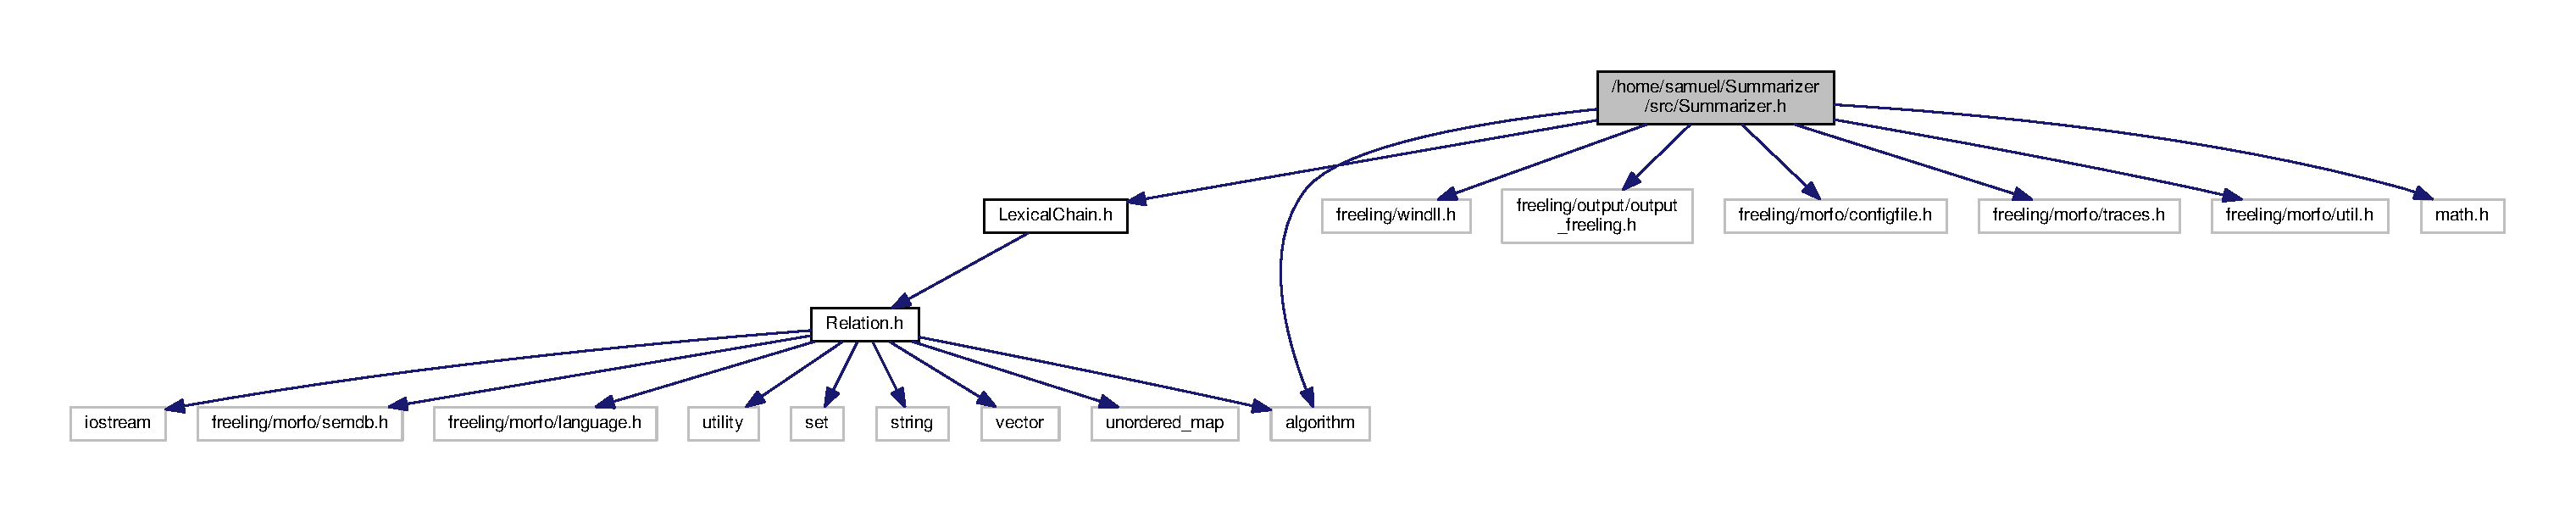
\includegraphics[width=350pt]{Summarizer_8h__incl}
\end{center}
\end{figure}
This graph shows which files directly or indirectly include this file\+:
\nopagebreak
\begin{figure}[H]
\begin{center}
\leavevmode
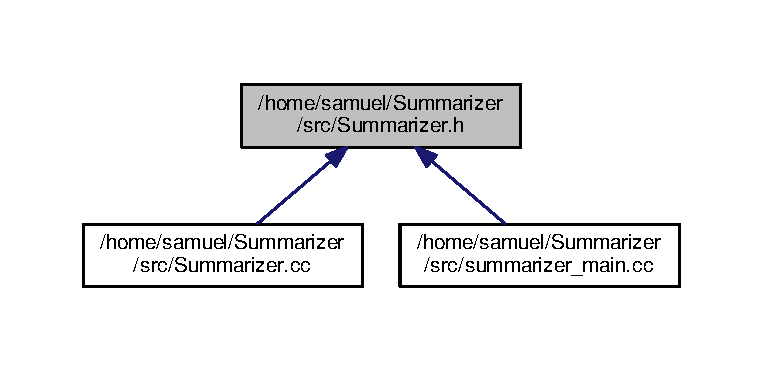
\includegraphics[width=288pt]{Summarizer_8h__dep__incl}
\end{center}
\end{figure}
\subsection*{Classes}
\begin{DoxyCompactItemize}
\item 
class \hyperlink{classSummarizer}{Summarizer}
\begin{DoxyCompactList}\small\item\em \hyperlink{classSummarizer}{Summarizer} class summarizes a document using the lexical chains method. \end{DoxyCompactList}\end{DoxyCompactItemize}
\subsection*{Macros}
\begin{DoxyCompactItemize}
\item 
\#define \hyperlink{Summarizer_8h_ab1e34bc45e4737f4c255db28d8616820}{M\+O\+D\+\_\+\+T\+R\+A\+C\+E\+N\+A\+M\+E}~L\char`\"{}A\+N\+A\+L\+Y\+Z\+E\+R\char`\"{}
\end{DoxyCompactItemize}


\subsection{Macro Definition Documentation}
\hypertarget{Summarizer_8h_ab1e34bc45e4737f4c255db28d8616820}{}\index{Summarizer.\+h@{Summarizer.\+h}!M\+O\+D\+\_\+\+T\+R\+A\+C\+E\+N\+A\+M\+E@{M\+O\+D\+\_\+\+T\+R\+A\+C\+E\+N\+A\+M\+E}}
\index{M\+O\+D\+\_\+\+T\+R\+A\+C\+E\+N\+A\+M\+E@{M\+O\+D\+\_\+\+T\+R\+A\+C\+E\+N\+A\+M\+E}!Summarizer.\+h@{Summarizer.\+h}}
\subsubsection[{M\+O\+D\+\_\+\+T\+R\+A\+C\+E\+N\+A\+M\+E}]{\setlength{\rightskip}{0pt plus 5cm}\#define M\+O\+D\+\_\+\+T\+R\+A\+C\+E\+N\+A\+M\+E~L\char`\"{}A\+N\+A\+L\+Y\+Z\+E\+R\char`\"{}}\label{Summarizer_8h_ab1e34bc45e4737f4c255db28d8616820}

\hypertarget{summarizer__main_8cc}{}\section{/home/samuel/\+Summarizer/src/summarizer\+\_\+main.cc File Reference}
\label{summarizer__main_8cc}\index{/home/samuel/\+Summarizer/src/summarizer\+\_\+main.\+cc@{/home/samuel/\+Summarizer/src/summarizer\+\_\+main.\+cc}}
{\ttfamily \#include \char`\"{}freeling/morfo/analyzer.\+h\char`\"{}}\\*
{\ttfamily \#include \char`\"{}freeling/morfo/util.\+h\char`\"{}}\\*
{\ttfamily \#include \char`\"{}config.\+h\char`\"{}}\\*
{\ttfamily \#include \char`\"{}Summarizer.\+h\char`\"{}}\\*
Include dependency graph for summarizer\+\_\+main.\+cc\+:
\nopagebreak
\begin{figure}[H]
\begin{center}
\leavevmode
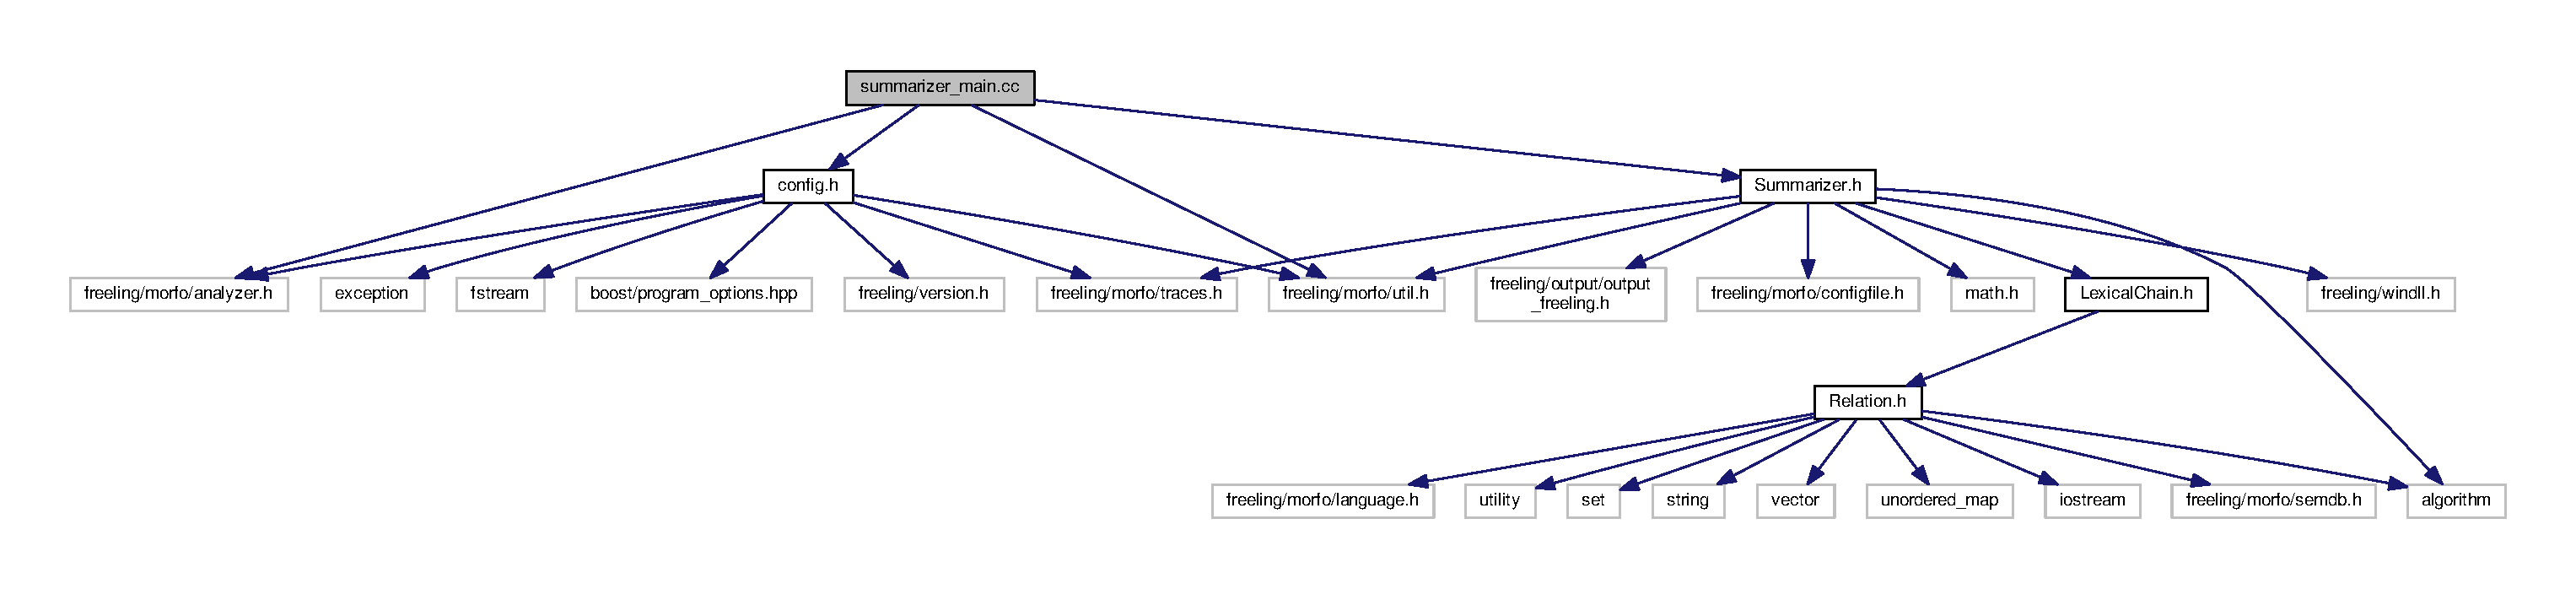
\includegraphics[width=350pt]{summarizer__main_8cc__incl}
\end{center}
\end{figure}
\subsection*{Functions}
\begin{DoxyCompactItemize}
\item 
analyzer\+::config\+\_\+options \hyperlink{summarizer__main_8cc_a70c445ce9ad7ae7b7331866c2afefdd1}{fill\+\_\+config} (const wstring \&path)
\begin{DoxyCompactList}\small\item\em predeclarations \end{DoxyCompactList}\item 
analyzer\+::invoke\+\_\+options \hyperlink{summarizer__main_8cc_a48711a601ad6eea7aafce73672db2024}{fill\+\_\+invoke} ()
\begin{DoxyCompactList}\small\item\em Load an ad-\/hoc set of invoke options. \end{DoxyCompactList}\item 
int \hyperlink{summarizer__main_8cc_a3c04138a5bfe5d72780bb7e82a18e627}{main} (int argc, char $\ast$$\ast$argv)
\end{DoxyCompactItemize}


\subsection{Function Documentation}
\hypertarget{summarizer__main_8cc_a70c445ce9ad7ae7b7331866c2afefdd1}{}\index{summarizer\+\_\+main.\+cc@{summarizer\+\_\+main.\+cc}!fill\+\_\+config@{fill\+\_\+config}}
\index{fill\+\_\+config@{fill\+\_\+config}!summarizer\+\_\+main.\+cc@{summarizer\+\_\+main.\+cc}}
\subsubsection[{fill\+\_\+config}]{\setlength{\rightskip}{0pt plus 5cm}analyzer\+::config\+\_\+options fill\+\_\+config (
\begin{DoxyParamCaption}
\item[{const wstring \&}]{path}
\end{DoxyParamCaption}
)}\label{summarizer__main_8cc_a70c445ce9ad7ae7b7331866c2afefdd1}


predeclarations 

Load an ad-\/hoc set of configuration options. Language of text to process

Tokenizer configuration file

Splitter configuration file

Morphological analyzer options

N\+E\+C config file

Sense annotator and W\+S\+D config files

Tagger options

Chart parser config file

Dependency parsers config files

Coreference resolution config file \hypertarget{summarizer__main_8cc_a48711a601ad6eea7aafce73672db2024}{}\index{summarizer\+\_\+main.\+cc@{summarizer\+\_\+main.\+cc}!fill\+\_\+invoke@{fill\+\_\+invoke}}
\index{fill\+\_\+invoke@{fill\+\_\+invoke}!summarizer\+\_\+main.\+cc@{summarizer\+\_\+main.\+cc}}
\subsubsection[{fill\+\_\+invoke}]{\setlength{\rightskip}{0pt plus 5cm}analyzer\+::invoke\+\_\+options fill\+\_\+invoke (
\begin{DoxyParamCaption}
{}
\end{DoxyParamCaption}
)}\label{summarizer__main_8cc_a48711a601ad6eea7aafce73672db2024}


Load an ad-\/hoc set of invoke options. 

Level of analysis in input and output

activate/deactivate morphological analyzer modules \hypertarget{summarizer__main_8cc_a3c04138a5bfe5d72780bb7e82a18e627}{}\index{summarizer\+\_\+main.\+cc@{summarizer\+\_\+main.\+cc}!main@{main}}
\index{main@{main}!summarizer\+\_\+main.\+cc@{summarizer\+\_\+main.\+cc}}
\subsubsection[{main}]{\setlength{\rightskip}{0pt plus 5cm}int main (
\begin{DoxyParamCaption}
\item[{int}]{argc, }
\item[{char $\ast$$\ast$}]{argv}
\end{DoxyParamCaption}
)}\label{summarizer__main_8cc_a3c04138a5bfe5d72780bb7e82a18e627}
read Free\+Ling installation path if given, use default otherwise

set config options (which modules to create, with which configuration)

create analyzer

set invoke options (which modules to use)

load invoke options into analyzer

load document to analyze

analyze text, leave result in doc

create summarizer

summarize document

print the summary 
%--- End generated contents ---

% Index
\backmatter
\newpage
\phantomsection
\clearemptydoublepage
\addcontentsline{toc}{chapter}{Index}
\printindex

\end{document}
